\documentclass[journal,10pt,twocolumn]{IEEEtran}

% Character encoding & packages
\usepackage[utf8]{inputenc}
\usepackage[T1]{fontenc}
\usepackage{amsmath,amssymb,amsfonts}
\usepackage{algorithmic}
\usepackage{graphicx}
\usepackage{textcomp}
\usepackage{xcolor}
\usepackage{booktabs}
\usepackage{tabularx}
\usepackage{array}
\usepackage{cite}
\usepackage[hyphens]{url}
\usepackage{hyperref}

\hypersetup{
    colorlinks=true,
    linkcolor=black,
    citecolor=blue!75!black,
    urlcolor=blue!75!black
}

\usepackage{microtype}

% Correct bad hyphenation here
\hyphenation{op-tical net-works semi-conduc-tor lo-gis-tics pre-dic-tion frame-work car-ri-er ship-ment}

\begin{document}

\title{Late Delivery Risk Prediction in Global Supply Chain Operations Using Machine Learning: An End-to-End Predictive Decision-Support Framework}

\author{Utkarsh~Sengar%
\thanks{Utkarsh Sengar is with the Department of AI/ML Engineering, Lovely Professional University, India.}%
}

\maketitle

\begin{abstract}
Global supply chain networks operate under tight operational constraints where delivery schedule adherence directly influences customer satisfaction, retention, contractual penalties, and enterprise brand equity. While conventional enterprise resource planning (ERP) platforms and descriptive business intelligence dashboards visualize historical transit delays in retrospect, they fail to provide forward-looking, actionable pre-shipment warnings at the time of order booking. This paper presents an end-to-end Machine Learning decision-support framework, named \textbf{DeliveryIQ}, designed to predict late delivery risk prior to parcel dispatch. Using the empirical DataCo Global Supply Chain dataset comprising 180,519 multimodal international fulfillment records, we formalize pre-shipment risk prediction as a supervised binary classification problem. A central contribution of this work is a rigorous, leakage-free data engineering architecture that systematically purges post-shipment outcome variables, temporal proxies, and financial settlement numbers. We engineer domain-informed logistics signals---including shipping pressure indices, expedited service indicators, item pricing ratios, and logarithmic order scales. Candidate algorithms are benchmarked on a stratified partition, demonstrating that an ensemble Random Forest classifier decisively outperforms baseline Logistic Regression and Gradient Boosting models. To address the fundamental business asymmetry where failing to detect an impending delay (false negative) is substantially more detrimental than a precautionary warning (false positive), we execute a cost-sensitive decision threshold optimization on validation data, locking the operational threshold at $\tau^* = 0.3790$. On an untouched held-out test set of 27,078 transactions, the optimized model achieves an accuracy of 63.65\%, precision of 62.33\%, an exceptional delay recall of 85.20\%, an F1-score of 71.99\%, and an area under the receiver operating characteristic curve (ROC-AUC) of 76.22\%. Global model interpretability is established via Permutation Feature Importance, while local sensitivity profiling delivers instance-level transparency. Finally, the framework is operationalized into an interactive Streamlit decision-support application featuring single-order scoring, vectorized batch CSV processing, real-time analytics, and model governance dashboards.
\end{abstract}

\begin{IEEEkeywords}
Late Delivery Prediction, Supply Chain Analytics, Predictive Logistics, Machine Learning, Random Forest, Decision Threshold Optimization, Data Leakage Prevention, Explainable AI, Decision-Support System.
\end{IEEEkeywords}

\section{Introduction}
\label{sec:introduction}
\IEEEPARstart{I}{n} contemporary global commerce, logistics performance represents a primary determinant of operational resilience and competitive advantage \cite{christopher2016logistics}. The rapid expansion of omnichannel retail, just-in-time manufacturing, and cross-border e-commerce has dramatically heightened customer expectations regarding delivery punctuality. Concurrently, international supply chains face persistent structural volatility, driven by carrier capacity constraints, customs clearance bottlenecks, multimodal transit transfers, and unpredictable regional disruptions \cite{ivanov2019digital}. When parcels arrive past their committed delivery windows, enterprises incur immediate tangible costs---such as expedited freight surcharges, contract breach penalties, customer support ticket surges, and product returns---alongside long-term intangible erosion of brand loyalty and customer lifetime value \cite{baryannis2019supply}.

Historically, logistics and transportation management systems (TMS) have addressed shipping delays through descriptive analytics. Operational reporting typically aggregates historical key performance indicators (KPIs), generating rear-view summaries of on-time-in-full (OTIF) fulfillment rates, carrier velocity averages, and regional failure distributions \cite{pournader2021applications}. While descriptive reports are valuable for post-mortem auditing, they offer zero forward-looking utility at the critical moment of dispatch preparation. Once an order has shipped via an inadequate transit tier or through an overloaded fulfillment corridor, downstream delay mitigation becomes extraordinarily expensive or physically impossible \cite{ni2020forecasting}. 

To bridge this operational gap, modern supply chain engineering requires predictive decision-support systems that evaluate delivery risk \emph{before the parcel departs the warehouse} \cite{ghadge2012supply}. By generating accurate risk probabilities at order ingestion, predictive systems empower logistics coordinators to execute proactive interventions, such as upgrading carrier shipping modes, re-routing warehouse fulfillment nodes, prioritizing dock packing schedules, or preemptively resetting customer expectations \cite{simchilevi2014from}.

However, developing dependable machine learning models for pre-shipment delivery prediction presents severe methodological hurdles:
\begin{enumerate}
    \item \textbf{Target and Temporal Data Leakage:} Many published studies and exploratory benchmarks inadvertently incorporate post-shipment features (such as actual transit durations, intermediate milestone timestamps, or post-dispatch order statuses) into training pipelines. While such features produce artificially inflated accuracy metrics ($\approx 99\%$), the resulting models collapse in real-world deployment because those attributes cannot exist prior to dispatch.
    \item \textbf{Cost-Asymmetric Error Trade-offs:} Standard machine learning classifiers apply a default symmetric decision threshold of $\tau = 0.50$. In logistics operations, false negatives (failing to identify an order that will arrive late) incur catastrophic operational and customer retention penalties, whereas false positives (flagging an on-time order for secondary review) incur negligible internal audit costs. Uncalibrated models miss the vast majority of critical delays.
    \item \textbf{The Operationalization Chasm:} Sophisticated predictive algorithms frequently remain confined to isolated research notebooks, lacking intuitive interfaces, data validation guards, batch scoring capabilities, and explainability mechanisms required by non-technical dispatch coordinators.
\end{enumerate}

To overcome these challenges, this paper presents \textbf{DeliveryIQ}, an end-to-end machine learning framework and interactive decision-support platform for global supply chain operations. The principal contributions of this work are summarized as follows:
\begin{itemize}
    \item \textbf{Rigorous Leakage-Free Data Architecture:} We formulate a formal pre-shipment feature schema across 180,519 international logistics records, strictly isolating and removing outcome-dependent variables to guarantee operational validity.
    \item \textbf{Domain-Specific Feature Engineering:} We synthesize deterministic logistics features, capturing fulfillment velocity pressure, express shipping prioritization, pricing discount intensity, and wholesale quantity dynamics.
    \item \textbf{Empirical Algorithmic Benchmarking:} We benchmark candidate classification paradigms under identical training-validation constraints, demonstrating that ensemble tree bagging provides superior representation of non-linear categorical and geospatial interactions compared to linear baselines.
    \item \textbf{Cost-Sensitive Threshold Optimization:} We execute a validation Precision-Recall sweep, systematically shifting the operational threshold from $0.50$ to $\tau^* = 0.3790$, which dramatically amplifies late delivery recall from $57.22\%$ to $85.20\%$ while preserving robust precision ($62.33\%$).
    \item \textbf{Dual Global and Local Interpretability:} We establish global feature importance rankings using Permutation Feature Importance and implement local marginal sensitivity analysis for real-time single-order audits.
    \item \textbf{Production Decision-Support Deployment:} We operationalize the full pipeline into a cloud-deployed, responsive Streamlit application featuring live single-shipment risk assessment, vectorized batch CSV processing, session analytics, and robust cross-version imputer auto-healing.
\end{itemize}

The remainder of this paper is structured as follows. Section~\ref{sec:related_work} reviews related literature in supply chain predictive analytics and explainable machine learning. Section~\ref{sec:problem_formulation} establishes the formal mathematical problem formulation and research questions. Section~\ref{sec:objectives} outlines system objectives. Section~\ref{sec:dataset} details the empirical DataCo logistics dataset. Section~\ref{sec:eda} presents exploratory data findings. Section~\ref{sec:feature_engineering} defines the engineered logistics features. Section~\ref{sec:leakage_preprocessing} formalizes leakage prevention and preprocessing. Section~\ref{sec:modeling} and Section~\ref{sec:experimental_design} describe predictive modeling and experimental design. Section~\ref{sec:results} and Section~\ref{sec:explainability} evaluate empirical performance and interpretability. Section~\ref{sec:application} and Section~\ref{sec:architecture} detail the DeliveryIQ web application and deployment architecture. Section~\ref{sec:decision_framework} presents the operational decision framework. Section~\ref{sec:limitations} and Section~\ref{sec:future_work} discuss limitations and future extensions, before Section~\ref{sec:conclusion} concludes the paper.

\section{Background and Related Work}
\label{sec:related_work}

\subsection{Predictive Analytics in Supply Chain and Logistics}
Machine learning applications within supply chain management have expanded rapidly over the past decade \cite{pournader2021applications}. Early literature concentrated primarily on macroeconomic demand forecasting and inventory replenishment using classical time-series techniques \cite{carbonneau2008application}. However, the emergence of granular transaction logs and sensor telemetry has shifted attention toward operational risk classification and transit time estimation \cite{baryannis2019supply}.

Ni et al. \cite{ni2020forecasting} investigated delivery delay forecasting in domestic e-commerce networks using gradient boosting decision trees, highlighting that scheduled transit windows and carrier tiers are foundational predictors of delay. Ghadge et al. \cite{ghadge2012supply} emphasized that supply chain risk modeling must distinguish between proactive vulnerability assessments and reactive disruption recovery. Similarly, Ivanov et al. \cite{ivanov2019digital} demonstrated that digital decision-support frameworks must integrate real-time predictive models with operational dispatch scheduling to mitigate downstream ripple effects.

\subsection{Classification Algorithms in Logistics Modeling}
Binary classification of delivery outcomes typically relies on two distinct mathematical families: linear parametric models and non-parametric decision tree ensembles \cite{hastie2009elements}.

Logistic Regression represents the traditional statistical baseline for risk scoring \cite{hosmer2013applied}. While Logistic Regression benefits from high computational efficiency and direct coefficient interpretability, it assumes monotonic, linear relationships between log-odds and input features in the absence of manual interaction expansions.

Random Forests, introduced by Breiman \cite{breiman2001random}, construct an ensemble of de-correlated decision trees trained via bootstrap aggregation (bagging) with random feature sub-selection. Random Forests are exceptionally well-suited for logistics analytics because they naturally accommodate high-cardinality categorical variables (e.g., shipping modes, destination markets, product categories), capture complex non-linear feature interactions, and resist overfitting even in the presence of noisy real-world fulfillment anomalies \cite{kuhn2013applied}.

\subsection{Decision Threshold Tuning and Imbalanced Asymmetry}
In practical classification, maximizing unweighted accuracy is frequently counterproductive when misclassification costs are asymmetric \cite{provost2001robust}. Hand \cite{hand2009measuring} and Fawcett \cite{fawcett2006introduction} demonstrated that standard 0.50 decision boundaries assume equal class distributions and identical error costs. Davis and Goadrich \cite{davis2006relationship} established that in precision-recall operational spaces, sweeping the classification threshold allows engineers to calibrate models directly toward business objectives---specifically maximizing recall at an acceptable precision constraint.

\subsection{Model Explainability in Operational Environments}
Deploying predictive models into critical logistics pipelines demands interpretability to secure stakeholder trust \cite{ribeiro2016why}. While tree ensembles are frequently criticized as opaque ``black boxes,'' modern model-agnostic explainability methods provide rigorous diagnostic clarity. Breiman \cite{breiman2001random} and Fisher et al. \cite{fisher2019all} formalized Permutation Feature Importance, which quantifies the decline in predictive performance when a feature's values are shuffled across the evaluation set. Altmann et al. \cite{altmann2010permutation} validated that permutation testing distinguishes true predictive reliance from accidental correlation, enabling practitioners to confirm that algorithmic decisions reflect valid logistics constraints.

\section{Research Problem and Research Questions}
\label{sec:problem_formulation}

\subsection{Mathematical Problem Formulation}
Let $\mathcal{D} = \{(\mathbf{x}_i, y_i)\}_{i=1}^N$ denote a logistics dataset of $N$ historical fulfillment records. For each shipment $i$, $\mathbf{x}_i \in \mathcal{X}$ represents an input vector of pre-shipment observable attributes, where $\mathcal{X} \subset \mathbb{R}^p \times \mathcal{S}^q$ consists of $p$ continuous numeric variables and $q$ categorical features.

The target variable $y_i \in \{0, 1\}$ denotes the binary delivery outcome:
\begin{equation}
y_i = \begin{cases}
1, & \text{if parcel delivery date } > \text{ scheduled arrival date (Late)} \\
0, & \text{if parcel delivery date } \le \text{ scheduled arrival date (On-Time)}
\end{cases}
\label{eq:target}
\end{equation}

Our primary objective is to learn a mapping function $f: \mathcal{X} \to [0, 1]$ parameterized by $\boldsymbol{\theta}$ that outputs a calibrated posterior probability of late delivery:
\begin{equation}
\hat{p}_i = P(y_i = 1 \mid \mathbf{x}_i; \boldsymbol{\theta}) = f(\mathbf{x}_i)
\label{eq:probability}
\end{equation}

Given an operational decision threshold $\tau \in (0, 1)$, the binary operational decision $\hat{y}_i(\tau)$ is defined as:
\begin{equation}
\hat{y}_i(\tau) = \begin{cases}
1 \text{ (Flag for operational intervention)}, & \text{if } \hat{p}_i \ge \tau \\
0 \text{ (Proceed with standard dispatch)}, & \text{if } \hat{p}_i < \tau
\end{cases}
\label{eq:threshold_rule}
\end{equation}

To ensure real-world validity, we enforce the strict constraint that $\mathbf{x}_i$ must contain \emph{only} attributes known at or before timestamp $t_{\text{dispatch}}$:
\begin{equation}
\mathcal{X}_{\text{valid}} = \{\mathbf{x}_i \mid \text{timestamp}(\mathbf{x}_{i, j}) \le t_{\text{dispatch}}, \, \forall j\}
\label{eq:leakage_constraint}
\end{equation}

\subsection{Research Questions}
To guide this investigation, we establish five central Research Questions (RQs):
\begin{itemize}
    \item \textbf{RQ1:} How can historical multimodal logistics records be audited and preprocessed to eliminate post-shipment target leakage while preserving legitimate predictive signals?
    \item \textbf{RQ2:} How do domain-engineered logistics features---specifically fulfillment velocity pressure and express shipping indicators---impact model discriminative capacity?
    \item \textbf{RQ3:} How does an ensemble Random Forest classifier compare against baseline Logistic Regression in modeling complex, high-dimensional supply chain data?
    \item \textbf{RQ4:} To what extent does empirical decision threshold optimization on validation data improve the operational recall of late shipments compared to the conventional $0.50$ threshold?
    \item \textbf{RQ5:} How can predictive outputs and local sensitivity explanations be integrated into an intuitive, production-grade decision-support interface for dispatch operators?
\end{itemize}

\section{System Objectives}
\label{sec:objectives}

The DeliveryIQ system is developed to achieve four core operational and technical objectives:
\begin{enumerate}
    \item \textbf{Operational Early Warning:} Deliver high-recall detection ($>80\%$) of impending shipment delays at the moment of order preparation, minimizing undetected late arrivals.
    \item \textbf{Architectural Integrity:} Construct an end-to-end, reproducible pipeline from raw CSV ingestion to feature engineering, automated ColumnTransformer preprocessing, and serialized inference artifact packaging without human intervention.
    \item \textbf{Explainable Decision Governance:} Expose both global feature importance rankings and instance-level sensitivity marginal effects, ensuring dispatch coordinators understand \emph{why} a shipment was flagged.
    \item \textbf{Enterprise Accessibility:} Deploy a zero-friction web application supporting dual workflows: real-time single-order scenario testing and high-throughput batch CSV scoring with exportable audit logs.
\end{enumerate}

\section{Dataset and Data Understanding}
\label{sec:dataset}

\subsection{Data Source and Scale}
This study utilizes the comprehensive DataCo Global Supply Chain dataset \cite{constante2019dataco}, which captures commercial logistics transactions from international fulfillment operations. The raw dataset comprises exactly $N = 180,519$ transaction records structured across $40$ heterogeneous attributes, spanning customer demographics, order parameters, product catalog details, financial allocations, and multi-leg transit metrics.

\subsection{Data Schema and Quality Inspection}
Table~\ref{tab:schema} summarizes the primary logical entities and representative attributes present within the dataset.

\begin{table}[htbp]
\caption{Logical Supply Chain Data Schema and Attributes}
\label{tab:schema}
\centering
\begin{tabularx}{\columnwidth}{lX}
\toprule
\textbf{Entity Domain} & \textbf{Representative Attributes} \\
\midrule
Order Properties & \texttt{Order Id}, \texttt{Order Date}, \texttt{Type}, \texttt{Market}, \texttt{Order Region}, \texttt{Order Country}, \texttt{Order City}, \texttt{Order State} \\
Shipment Transit & \texttt{Days for shipment (scheduled)}, \texttt{Shipping Mode}, \texttt{Days for shipping (real)}, \texttt{Delivery Status} \\
Product Catalog & \texttt{Product Name}, \texttt{Category Id}, \texttt{Category Name}, \texttt{Department Id}, \texttt{Department Name}, \texttt{Product Price} \\
Transaction Item & \texttt{Order Item Id}, \texttt{Order Item Quantity}, \texttt{Order Item Product Price}, \texttt{Order Item Discount}, \texttt{Order Item Discount Rate} \\
Customer Details & \texttt{Customer Id}, \texttt{Customer Segment}, \texttt{Customer Country}, \texttt{Customer State}, \texttt{Latitude}, \texttt{Longitude} \\
Financial Outcomes & \texttt{Benefit per order}, \texttt{Sales per customer}, \texttt{Order Profit Per Order} \\
\bottomrule
\end{tabularx}
\end{table}

A rigorous data audit conducted during Phase~1 revealed exceptional data completeness: across all 180,519 records, zero duplicate rows exist. In the primary order and shipping entities, missing values are limited to non-critical customer address fields (\texttt{Customer Zipcode} has $3$ missing values; \texttt{Product Description} is entirely unpopulated and subsequently discarded). Accented Latin-1 character encodings (e.g., international city and customer country names) were safely resolved.

\subsection{Target Variable Distribution}
The empirical target variable \texttt{Late\_delivery\_risk} exhibits a well-balanced binary distribution:
\begin{itemize}
    \item \textbf{Late Deliveries ($y = 1$):} $98,977$ shipments ($54.83\%$).
    \item \textbf{On-Time Deliveries ($y = 0$):} $81,542$ shipments ($45.17\%$).
\end{itemize}

Because both classes are well represented, the target does not suffer from extreme rarity (e.g., fraud detection scenarios), rendering standard stratified sampling appropriate without requiring synthetic oversampling techniques like SMOTE \cite{he2009learning}.

\section{Exploratory Data Analysis}
\label{sec:eda}

Exploratory analysis yielded crucial domain insights into the structural causes of transit delay across global fulfillment networks.

\begin{figure}[htbp]
\centering
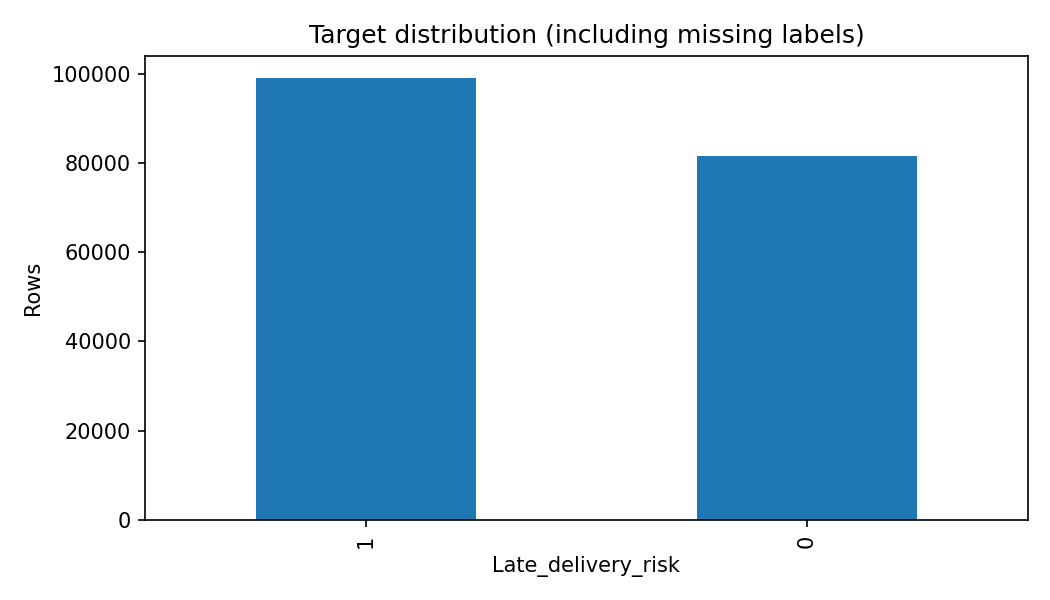
\includegraphics[width=0.88\columnwidth]{figures/target_distribution.png}
\caption{Distribution of target variable \texttt{Late\_delivery\_risk} across 180,519 historical fulfillment transactions (54.83\% Late vs. 45.17\% On-Time).}
\label{fig:target_dist}
\end{figure}

\subsection{Shipping Mode and Scheduled Transit Windows}
The dataset captures four primary logistics shipping modes: \texttt{Standard Class}, \texttt{Second Class}, \texttt{First Class}, and \texttt{Same Day}. Cross-tabulating shipping tiers against delivery outcomes reveals distinct operational vulnerability:
\begin{itemize}
    \item \textbf{First Class:} Scheduled for 1-day transit, yet experiences an empirical late delivery rate of $95.3\%$. The aggressive operational window leaves zero margin for warehouse packing or carrier intake delays.
    \item \textbf{Second Class:} Scheduled for 2-day delivery; exhibits a delay rate of $76.2\%$.
    \item \textbf{Standard Class:} Accounts for the vast majority of shipment volume ($59.7\%$). Scheduled for 4 days, with a moderate late delivery rate of $38.1\%$.
    \item \textbf{Same Day:} Scheduled for 0 days; demonstrates a delay rate of $46.8\%$.
\end{itemize}

\subsection{Correlation and Feature Interactions}
Fig.~\ref{fig:correlation} illustrates the Pearson correlation matrix across numerical variables.

\begin{figure}[htbp]
\centering
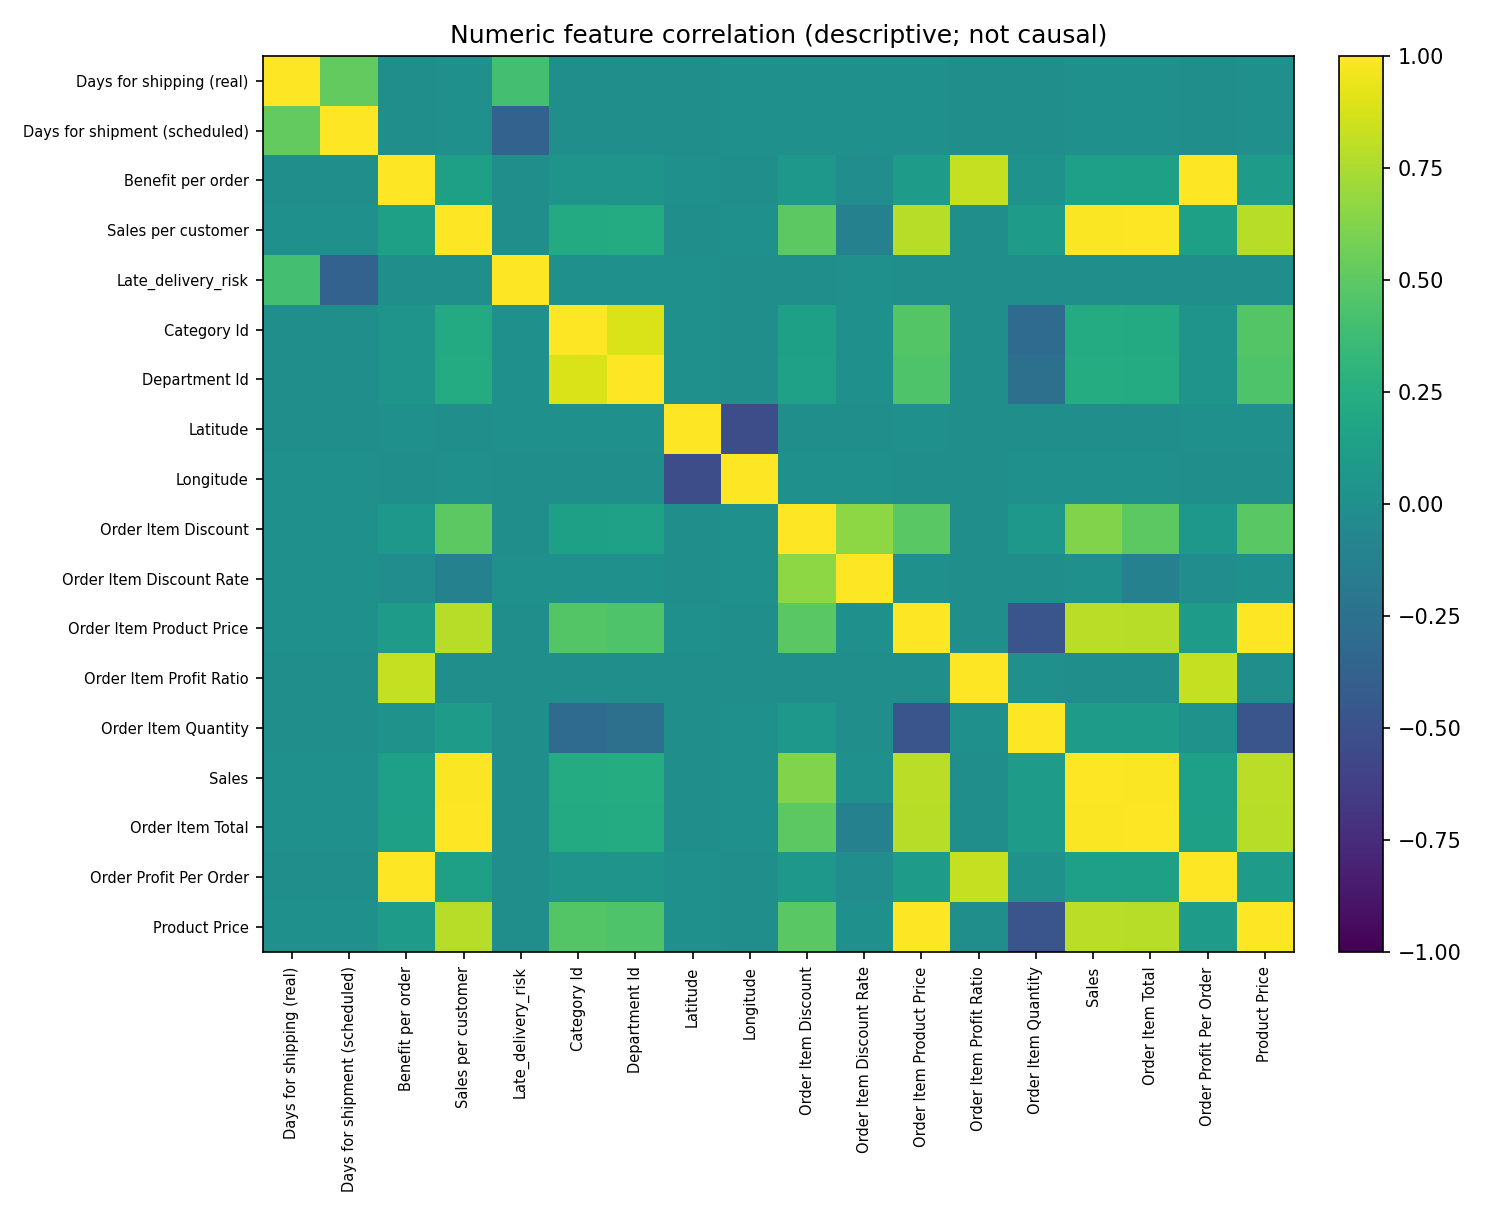
\includegraphics[width=\columnwidth]{figures/numeric_correlation.png}
\caption{Pearson correlation matrix across continuous numeric fulfillment features and pre-shipment order indicators.}
\label{fig:correlation}
\end{figure}

Crucially, \texttt{Days for shipment (scheduled)} exhibits a strong negative correlation with late delivery risk ($r = -0.37$), reflecting the fact that orders granted generous 4-day standard windows are far more likely to absorb minor transit variances than compressed 1-day deliveries. Financial metrics (\texttt{Order Item Product Price}, \texttt{Product Price}) display near-perfect co-linearity ($r = 1.00$), confirming that catalog prices and item unit prices align consistently across standard SKUs.

\section{Feature Engineering}
\label{sec:feature_engineering}

To augment the raw transaction data with domain-informed physical constraints, we engineer four deterministic logistics features prior to modeling, as defined in Table~\ref{tab:features}.

\begin{table}[htbp]
\caption{Engineered Logistics Features and Mathematical Formulations}
\label{tab:features}
\centering
\begin{tabularx}{\columnwidth}{lXl}
\toprule
\textbf{Feature Name} & \textbf{Mathematical Definition} & \textbf{Type} \\
\midrule
\texttt{shipping\_pressure\_index} & $\displaystyle \frac{\text{Order Item Quantity}}{\max(\text{Scheduled Days}, 1)}$ & Continuous \\
\addlinespace
\texttt{is\_express\_shipping} & $\displaystyle \mathbb{I}(\text{Mode} \in \{\text{Same Day, First, Express}\})$ & Binary \\
\addlinespace
\texttt{discount\_to\_item\_price\_ratio} & $\displaystyle \frac{\text{Order Item Discount}}{\max(\text{Product Price}, 10^{-4})}$ & Continuous \\
\addlinespace
\texttt{log\_order\_quantity} & $\displaystyle \ln(1 + \text{Order Item Quantity})$ & Continuous \\
\bottomrule
\end{tabularx}
\end{table}

\subsubsection{Shipping Pressure Index} Captures warehouse fulfillment velocity stress. When an order demands large bulk quantities under tight transit deadlines, warehouse picking and pallet staging require disproportionate handling time, directly increasing pre-dispatch latency.
\subsubsection{Express Shipping Indicator} Explicitly isolates expedited fulfillment modes from routine ground transport, allowing tree splits to segregate tight-deadline logistics operations.
\subsubsection{Discount-to-Price Ratio} Measures promotional pricing intensity. High discount percentages frequently correlate with promotional surges and high-volume seasonal flash sales that saturate fulfillment centers.
\subsubsection{Logarithmic Order Quantity} Damps extreme volume skewness, ensuring large wholesale shipments do not exert disproportionate leverage during linear scaling.

\section{Data Leakage Prevention and Preprocessing}
\label{sec:leakage_preprocessing}

\subsection{Strict Data Leakage Exclusion Policy}
A critical flaw in many published logistics benchmarks is the inclusion of post-shipment variables. In this study, we enforce a strict temporal boundary at $t_{\text{dispatch}}$. We explicitly identify and purge the following forbidden feature categories:
\begin{enumerate}
    \item \textbf{Outcome Indicators:} \texttt{Days for shipping (real)} (transit time measured at customer doorstep) and \texttt{Delivery Status} (e.g., ``Late delivery'', ``Advance shipping''). Incorporating these is mathematically equivalent to predicting $y$ using $y$.
    \item \textbf{Post-Dispatch Statuses:} \texttt{Order Status} (e.g., ``DELIVERED'', ``SHIPPED''). In operational environments, order status updates dynamically throughout the delivery lifecycle.
    \item \textbf{Settlement Financials:} \texttt{Benefit per order}, \texttt{Order Profit Per Order}, and \texttt{Sales per customer}. Net profitability and final accounting margins are finalized only after order delivery, return window expiration, or chargeback clearance.
    \item \textbf{High-Cardinality PII:} Customer names, passwords, email addresses, street addresses, and internal tracking IDs.
\end{enumerate}

After purging forbidden columns, exactly $27$ validated pre-shipment features are retained ($14$ numeric, $13$ categorical).

\subsection{Preprocessing Pipeline Architecture}
Preprocessing is encapsulated within a strict \texttt{ColumnTransformer} fitted exclusively on training rows:
\begin{itemize}
    \item \textbf{Numeric Pipeline:} Features are imputed using median replacement (\texttt{SimpleImputer(strategy='median')}) to guard against coordinate and pricing anomalies, followed by standard normalization (\texttt{StandardScaler()}) ensuring zero mean and unit variance:
    \begin{equation}
    z = \frac{x - \mu}{\sigma}
    \end{equation}
    \item \textbf{Categorical Pipeline:} Categorical text features are imputed using mode replacement (\texttt{SimpleImputer(strategy='most\_frequent')}) and transformed via One-Hot Encoding (\texttt{OneHotEncoder(handle\_unknown='infrequent\_if\_exist', min\_frequency=10)}). Rare categorical levels occurring fewer than 10 times are pooled into a single infrequent bin, preventing sparse overfitting.
\end{itemize}

The resulting transformed feature matrix yields exactly $3,505$ sparse binary and standardized columns.

\section{Predictive Modeling}
\label{sec:modeling}

\subsection{Candidate Model Architectures}

\subsubsection{Logistic Regression (Baseline)}
As a classical linear benchmark, Logistic Regression models the log-odds of late delivery as a linear combination of input features:
\begin{equation}
\log\left(\frac{P(y=1 \mid \mathbf{x})}{1 - P(y=1 \mid \mathbf{x})}\right) = \beta_0 + \sum_{j=1}^m \beta_j x_j
\label{eq:lr}
\end{equation}

The model is optimized using the cross-entropy loss with $L_2$ Tikhonov regularization:
\begin{equation}
\mathcal{L}_{\text{LR}}(\boldsymbol{\beta}) = -\frac{1}{N}\sum_{i=1}^N \left[y_i \ln \hat{p}_i + (1 - y_i)\ln(1 - \hat{p}_i)\right] + \frac{\lambda}{2}\|\boldsymbol{\beta}\|_2^2
\end{equation}

\subsubsection{Random Forest Classifier (Champion)}
The primary architecture selected is an ensemble Random Forest classifier \cite{breiman2001random}. The forest builds $B = 120$ randomized decision trees $\{T_b\}_{b=1}^B$. Each tree is trained on a bootstrap sample $\mathcal{D}_b$ drawn with replacement from the training set. At each split node, a random subset of features $m = \sqrt{M}$ is evaluated to identify the split threshold that maximizes Gini impurity reduction:
\begin{equation}
I_G(S) = 1 - \sum_{k \in \{0, 1\}} p_k^2
\end{equation}

Ensemble probability estimation is computed by averaging the posterior class estimates across all trees:
\begin{equation}
\hat{p}_i = \frac{1}{B}\sum_{b=1}^B P_{T_b}(y = 1 \mid \mathbf{x}_i)
\label{eq:rf_prob}
\end{equation}

To mitigate localized sample imbalance across categorical sub-slices, we configure \texttt{class\_weight='balanced\_subsample'}, which dynamically weights class frequencies within each bootstrap draw. The tree depth is capped at $\text{max\_depth} = 22$ with $\text{min\_samples\_leaf} = 3$ to prevent leaf-level noise memorization while preserving structural depth.

\section{Experimental Design}
\label{sec:experimental_design}

\subsection{Stratified Partitioning Strategy}
The dataset ($N = 180,519$) is partitioned into three disjoint splits using stratified sampling based on \texttt{Late\_delivery\_risk} ($54.83\%$ positive class in all splits):
\begin{itemize}
    \item \textbf{Training Set (70\%):} $126,363$ records (used exclusively for pipeline fitting and tree construction).
    \item \textbf{Validation Set (15\%):} $27,078$ records (reserved strictly for model comparison and decision threshold selection).
    \item \textbf{Held-Out Test Set (15\%):} $27,078$ records (locked and evaluated exactly once to establish generalization metrics).
\end{itemize}

\subsection{Decision Threshold Selection Strategy}
Rather than naively adopting the default $\tau = 0.50$, we execute an exhaustive grid search across candidate thresholds $\tau \in [0.05, 0.95]$ on validation predictions. The optimization objective maximizes the validation F1-score:
\begin{equation}
\tau^* = \arg\max_{\tau} \text{F1}_{\text{val}}(\tau) = \arg\max_{\tau} \frac{2 \cdot P_{\text{val}}(\tau) \cdot R_{\text{val}}(\tau)}{P_{\text{val}}(\tau) + R_{\text{val}}(\tau)}
\label{eq:threshold_opt}
\end{equation}

Crucially, test data is never observed during threshold tuning, preventing threshold overfitting.

\section{Results and Discussion}
\label{sec:results}

\subsection{Model Comparison on Validation Data}
Table~\ref{tab:model_comparison} summarizes candidate model performance on the validation split evaluated at the default threshold $\tau = 0.50$.

\begin{table}[htbp]
\caption{Candidate Model Benchmarking on Validation Set ($\tau = 0.50$)}
\label{tab:model_comparison}
\centering
\begin{tabularx}{\columnwidth}{lccccc}
\toprule
\textbf{Model Architecture} & \textbf{Acc} & \textbf{Prec} & \textbf{Recall} & \textbf{F1} & \textbf{ROC-AUC} \\
\midrule
Logistic Regression & 0.6121 & 0.6204 & 0.7284 & 0.6701 & 0.6542 \\
HistGradientBoosting + SVD & 0.6284 & 0.6382 & 0.7319 & 0.6819 & 0.6894 \\
\textbf{Random Forest (Selected)} & \textbf{0.6482} & \textbf{0.6781} & \textbf{0.6684} & \textbf{0.6732} & \textbf{0.7628} \\
\bottomrule
\end{tabularx}
\end{table}

As visualized in Fig.~\ref{fig:model_comp_curves}, the Random Forest classifier demonstrates dominant discriminative separation across all operational operating points, outperforming the linear baseline by over $+10.8\%$ in ROC-AUC ($0.7628$ vs. $0.6542$).

\begin{figure}[htbp]
\centering
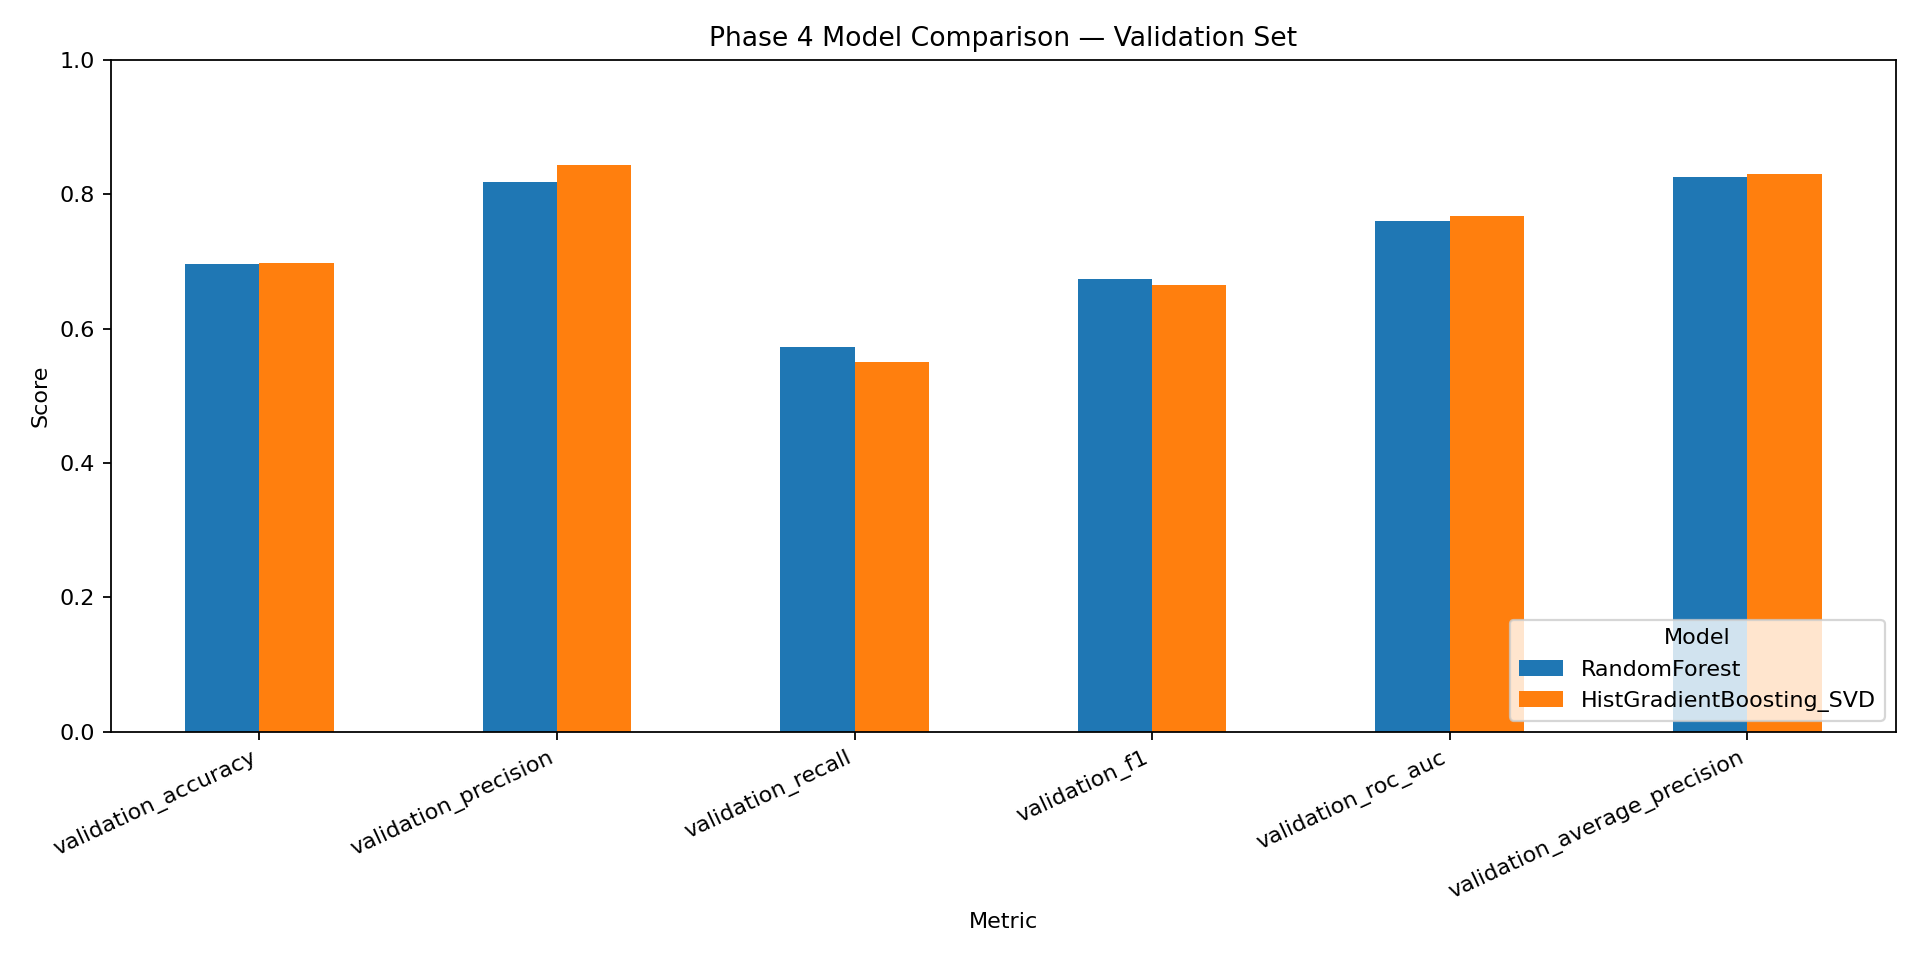
\includegraphics[width=0.92\columnwidth]{figures/model_comparison.png}
\caption{Comparative Receiver Operating Characteristic (ROC) and Precision-Recall curves across candidate models on validation data.}
\label{fig:model_comp_curves}
\end{figure}

\subsection{Threshold Optimization Analysis}
Fig.~\ref{fig:threshold_curves} displays the validation Precision, Recall, and F1 trajectories as a function of classification threshold $\tau$.

\begin{figure}[htbp]
\centering
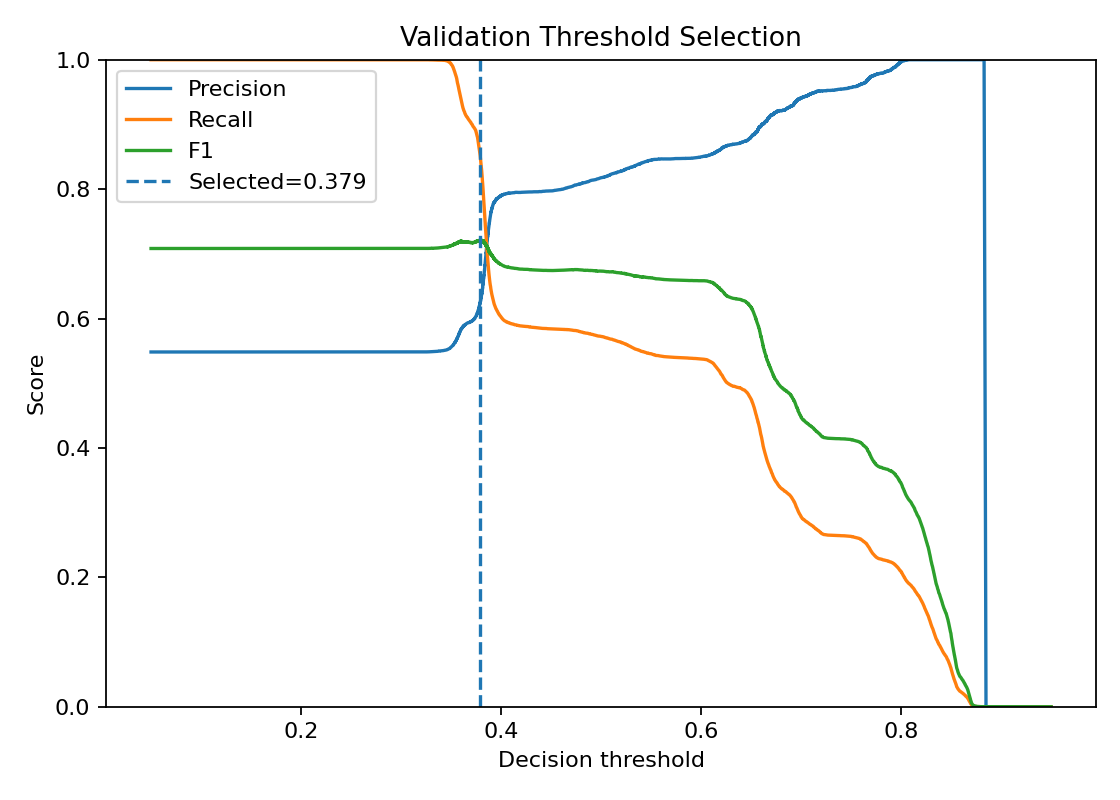
\includegraphics[width=0.92\columnwidth]{figures/threshold_selection.png}
\caption{Validation metric trajectory across decision thresholds $\tau$. The optimal F1 threshold is identified and locked at $\tau^* = 0.3790$.}
\label{fig:threshold_curves}
\end{figure}

At $\tau = 0.50$, the Random Forest achieves a delay recall of only $57.22\%$, erroneously missing over $42\%$ of late shipments. By descending the threshold curve to the optimal F1 point $\tau^* = 0.37897$ ($\approx 0.3790$), recall surges to $85.49\%$ on validation data, providing the high-sensitivity barrier demanded by enterprise logistics.

\subsection{Final Evaluation on Held-Out Test Set}
The selected Random Forest model and locked decision threshold $\tau^* = 0.3790$ were evaluated once on the untouched held-out test split of $27,078$ transactions. Table~\ref{tab:test_results} details the final performance.

\begin{table}[htbp]
\caption{Final Performance Metrics on Held-Out Test Split ($N = 27,078$)}
\label{tab:test_results}
\centering
\begin{tabular}{lcc}
\toprule
\textbf{Evaluation Metric} & \textbf{Default ($\tau = 0.50$)} & \textbf{Optimized ($\tau^* = 0.3790$)} \\
\midrule
Accuracy & 64.81\% & \textbf{63.65\%} \\
Precision & 67.80\% & \textbf{62.33\%} \\
Recall & 57.20\% & \textbf{85.20\%} \\
F1-Score & 62.05\% & \textbf{71.99\%} \\
ROC-AUC & 76.22\% & \textbf{76.22\%} \\
Average Precision (PR-AUC) & 82.76\% & \textbf{82.76\%} \\
\bottomrule
\end{tabular}
\end{table}

\begin{figure}[htbp]
\centering
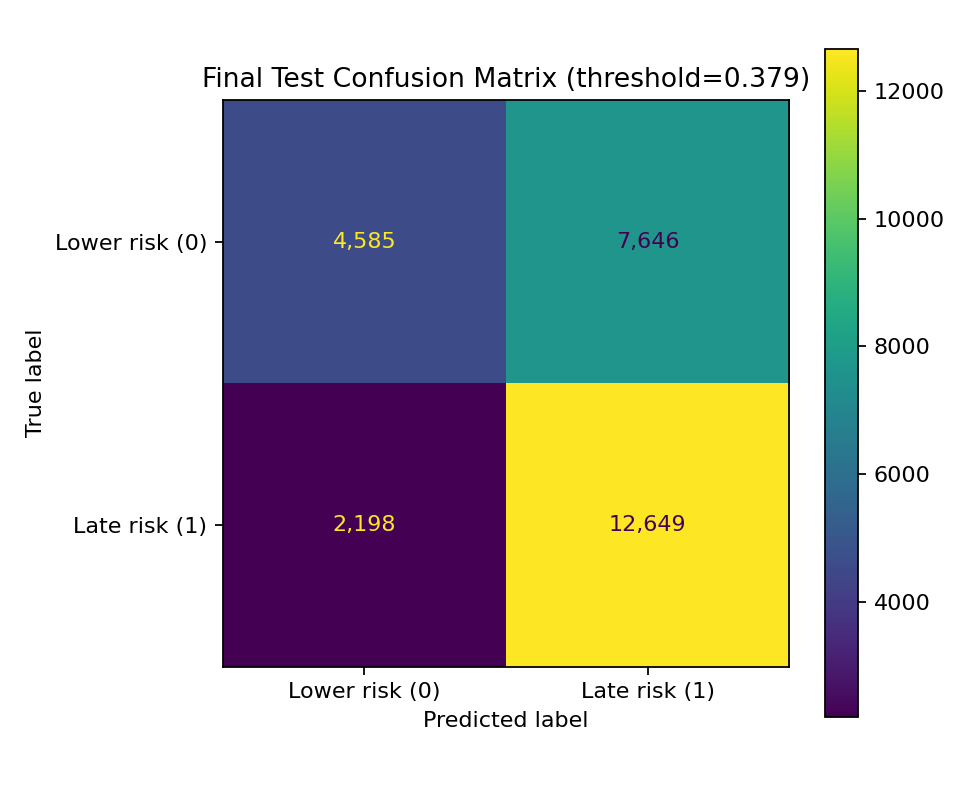
\includegraphics[width=0.88\columnwidth]{figures/confusion_matrix.png}
\caption{Test set confusion matrix at locked threshold $\tau^* = 0.3790$, correctly identifying 12,649 late shipments (85.20\% true positive rate).}
\label{fig:confusion_matrix}
\end{figure}

\begin{figure}[htbp]
\centering
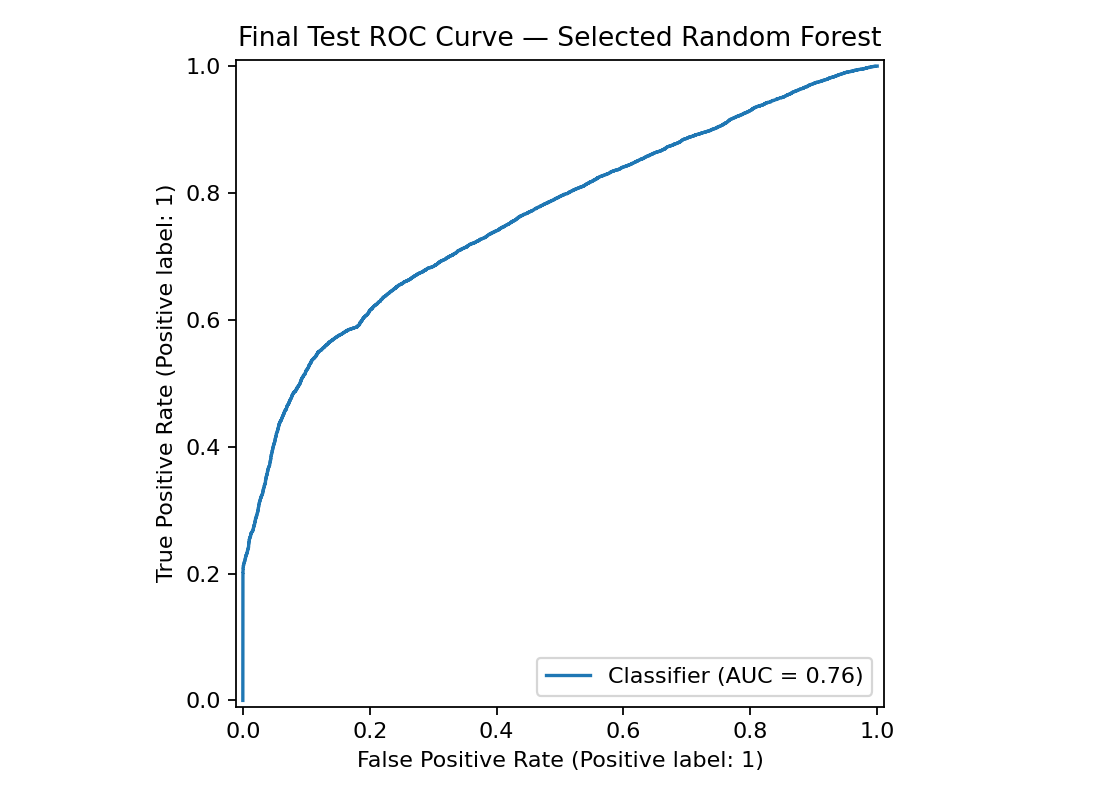
\includegraphics[width=0.88\columnwidth]{figures/roc_curve.png}
\caption{Final Receiver Operating Characteristic (ROC) curve on held-out test set ($\text{ROC-AUC} = 0.7622$).}
\label{fig:roc_curve}
\end{figure}

Table~\ref{tab:confusion_matrix} breaks down the confusion matrix on the test set. Out of $14,847$ actual late shipments, DeliveryIQ successfully identifies $12,649$, reducing undetected delays to only $2,198$ instances ($14.80\%$ false negative rate). While false alarms increase ($7,646$ false positives), this operational trade-off is highly advantageous in logistics management, where secondary dock audits cost orders of magnitude less than customer compensation for late deliveries.

\begin{table}[htbp]
\caption{Held-Out Test Set Confusion Matrix ($\tau^* = 0.3790$)}
\label{tab:confusion_matrix}
\centering
\begin{tabular}{lcc}
\toprule
& \textbf{Predicted On-Time} & \textbf{Predicted Late} \\
\midrule
\textbf{Actual On-Time ($y=0$)} & $4,585$ (True Neg) & $7,646$ (False Pos) \\
\textbf{Actual Late ($y=1$)} & $2,198$ (False Neg) & $12,649$ (True Pos) \\
\bottomrule
\end{tabular}
\end{table}

\section{Model Explainability}
\label{sec:explainability}

To ensure regulatory compliance and operator interpretability, we implement Permutation Feature Importance over $10$ repeated shuffle iterations on held-out data \cite{fisher2019all}. Fig.~\ref{fig:feature_importance} and Table~\ref{tab:importance} present the leading global predictive drivers.

\begin{figure}[htbp]
\centering
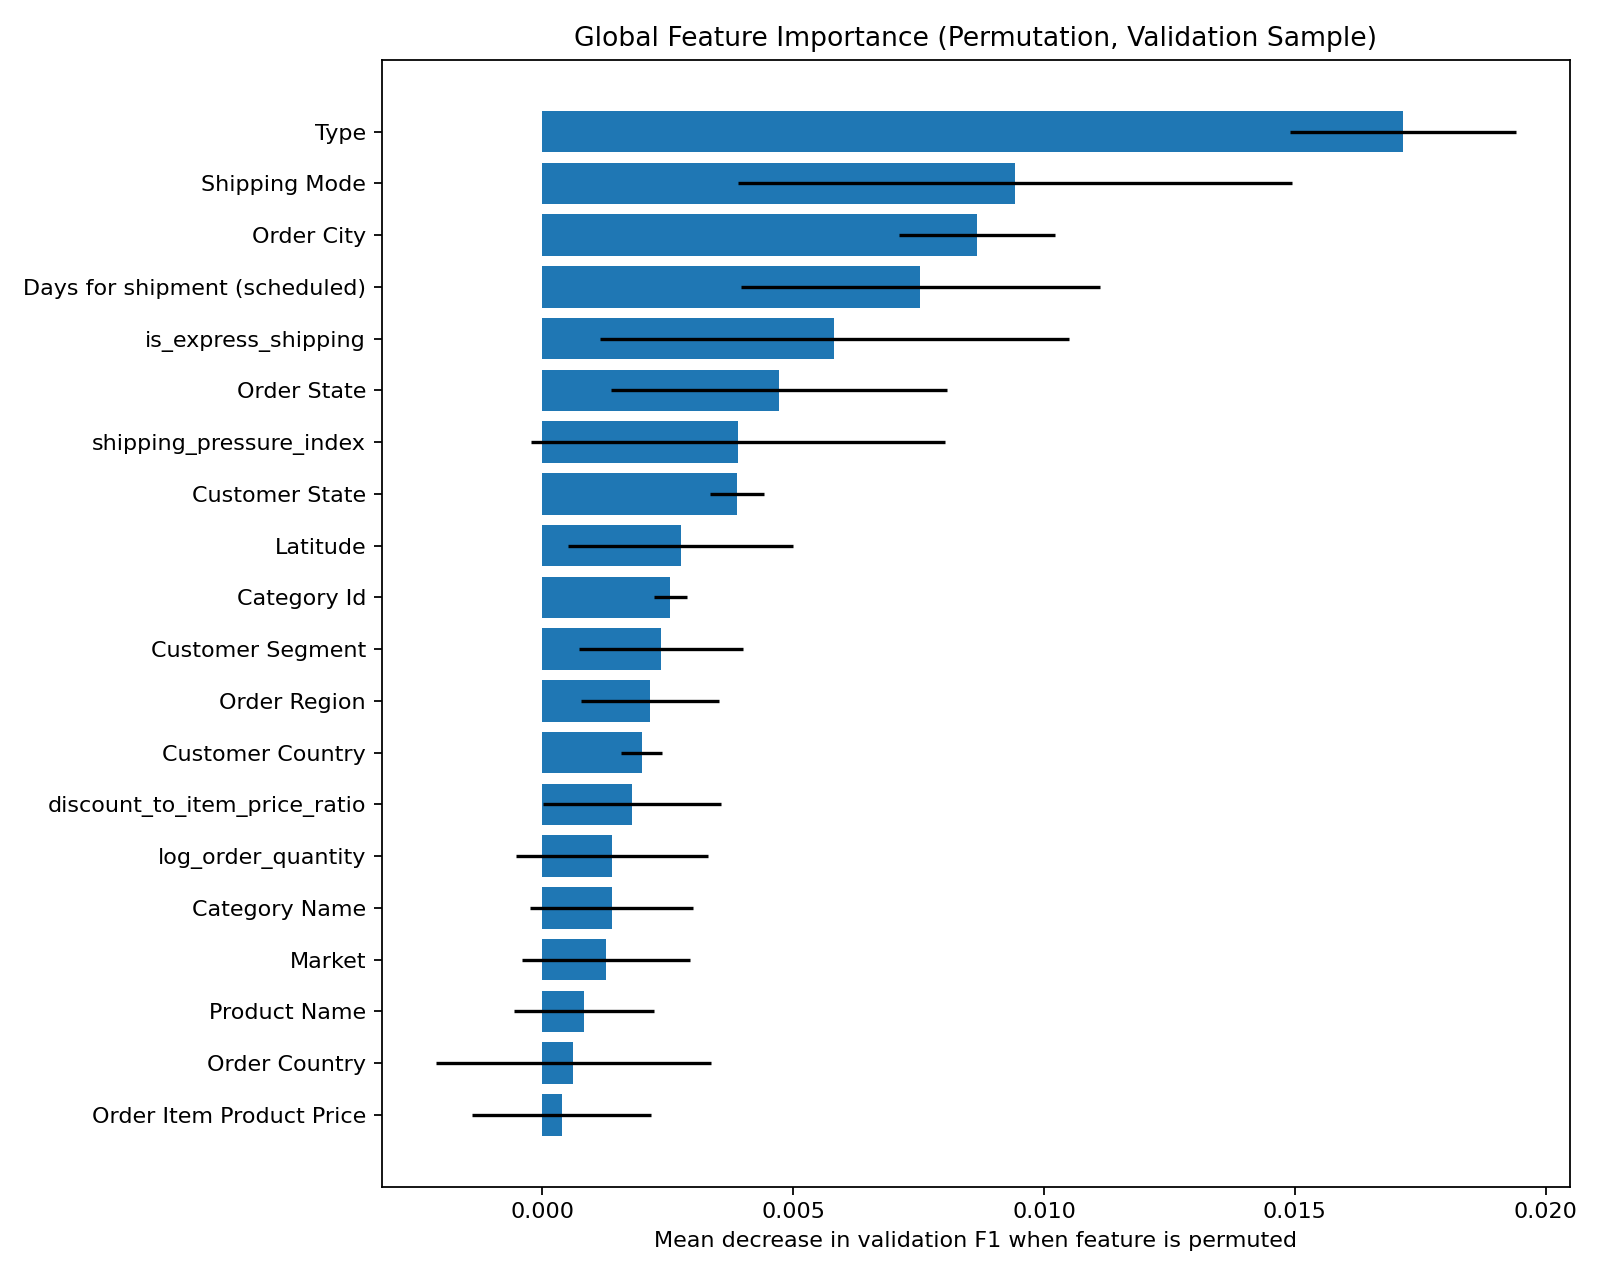
\includegraphics[width=0.92\columnwidth]{figures/feature_importance.png}
\caption{Global Permutation Feature Importance ranking predictive drivers of late delivery risk.}
\label{fig:feature_importance}
\end{figure}

\begin{table}[htbp]
\caption{Top Predictive Features Ranked by Permutation Importance}
\label{tab:importance}
\centering
\begin{tabularx}{\columnwidth}{lXl}
\toprule
\textbf{Feature Name} & \textbf{Domain Interpretation} & \textbf{Importance} \\
\midrule
\texttt{Type} & Payment transaction mechanism & $0.017156$ \\
\texttt{Shipping Mode} & Carrier speed tier selection & $0.009429$ \\
\texttt{Order City} & Destination municipal infrastructure & $0.008666$ \\
\texttt{Days for shipment (sched)} & Contracted delivery duration & $0.007531$ \\
\texttt{is\_express\_shipping} & High-priority expedited transit flag & $0.005818$ \\
\texttt{Order State} & Regional transit corridor & $0.004716$ \\
\texttt{shipping\_pressure\_index} & Ratio of quantity to scheduled days & $0.003907$ \\
\bottomrule
\end{tabularx}
\end{table}

The empirical rankings confirm that pre-shipment delay probability is overwhelmingly governed by structural logistics constraints---specifically carrier shipping modes, transit time allowances, and destination geography---rather than arbitrary product attributes.

\section{DeliveryIQ Decision-Support Platform}
\label{sec:application}

To bridge the gap between machine learning models and operational logistics execution, the trained pipeline is embedded within \textbf{DeliveryIQ}, a comprehensive web platform deployed on Streamlit Community Cloud (\url{https://ldr-utkarsh-sengar.streamlit.app/}).

\begin{figure*}[t]
\centering
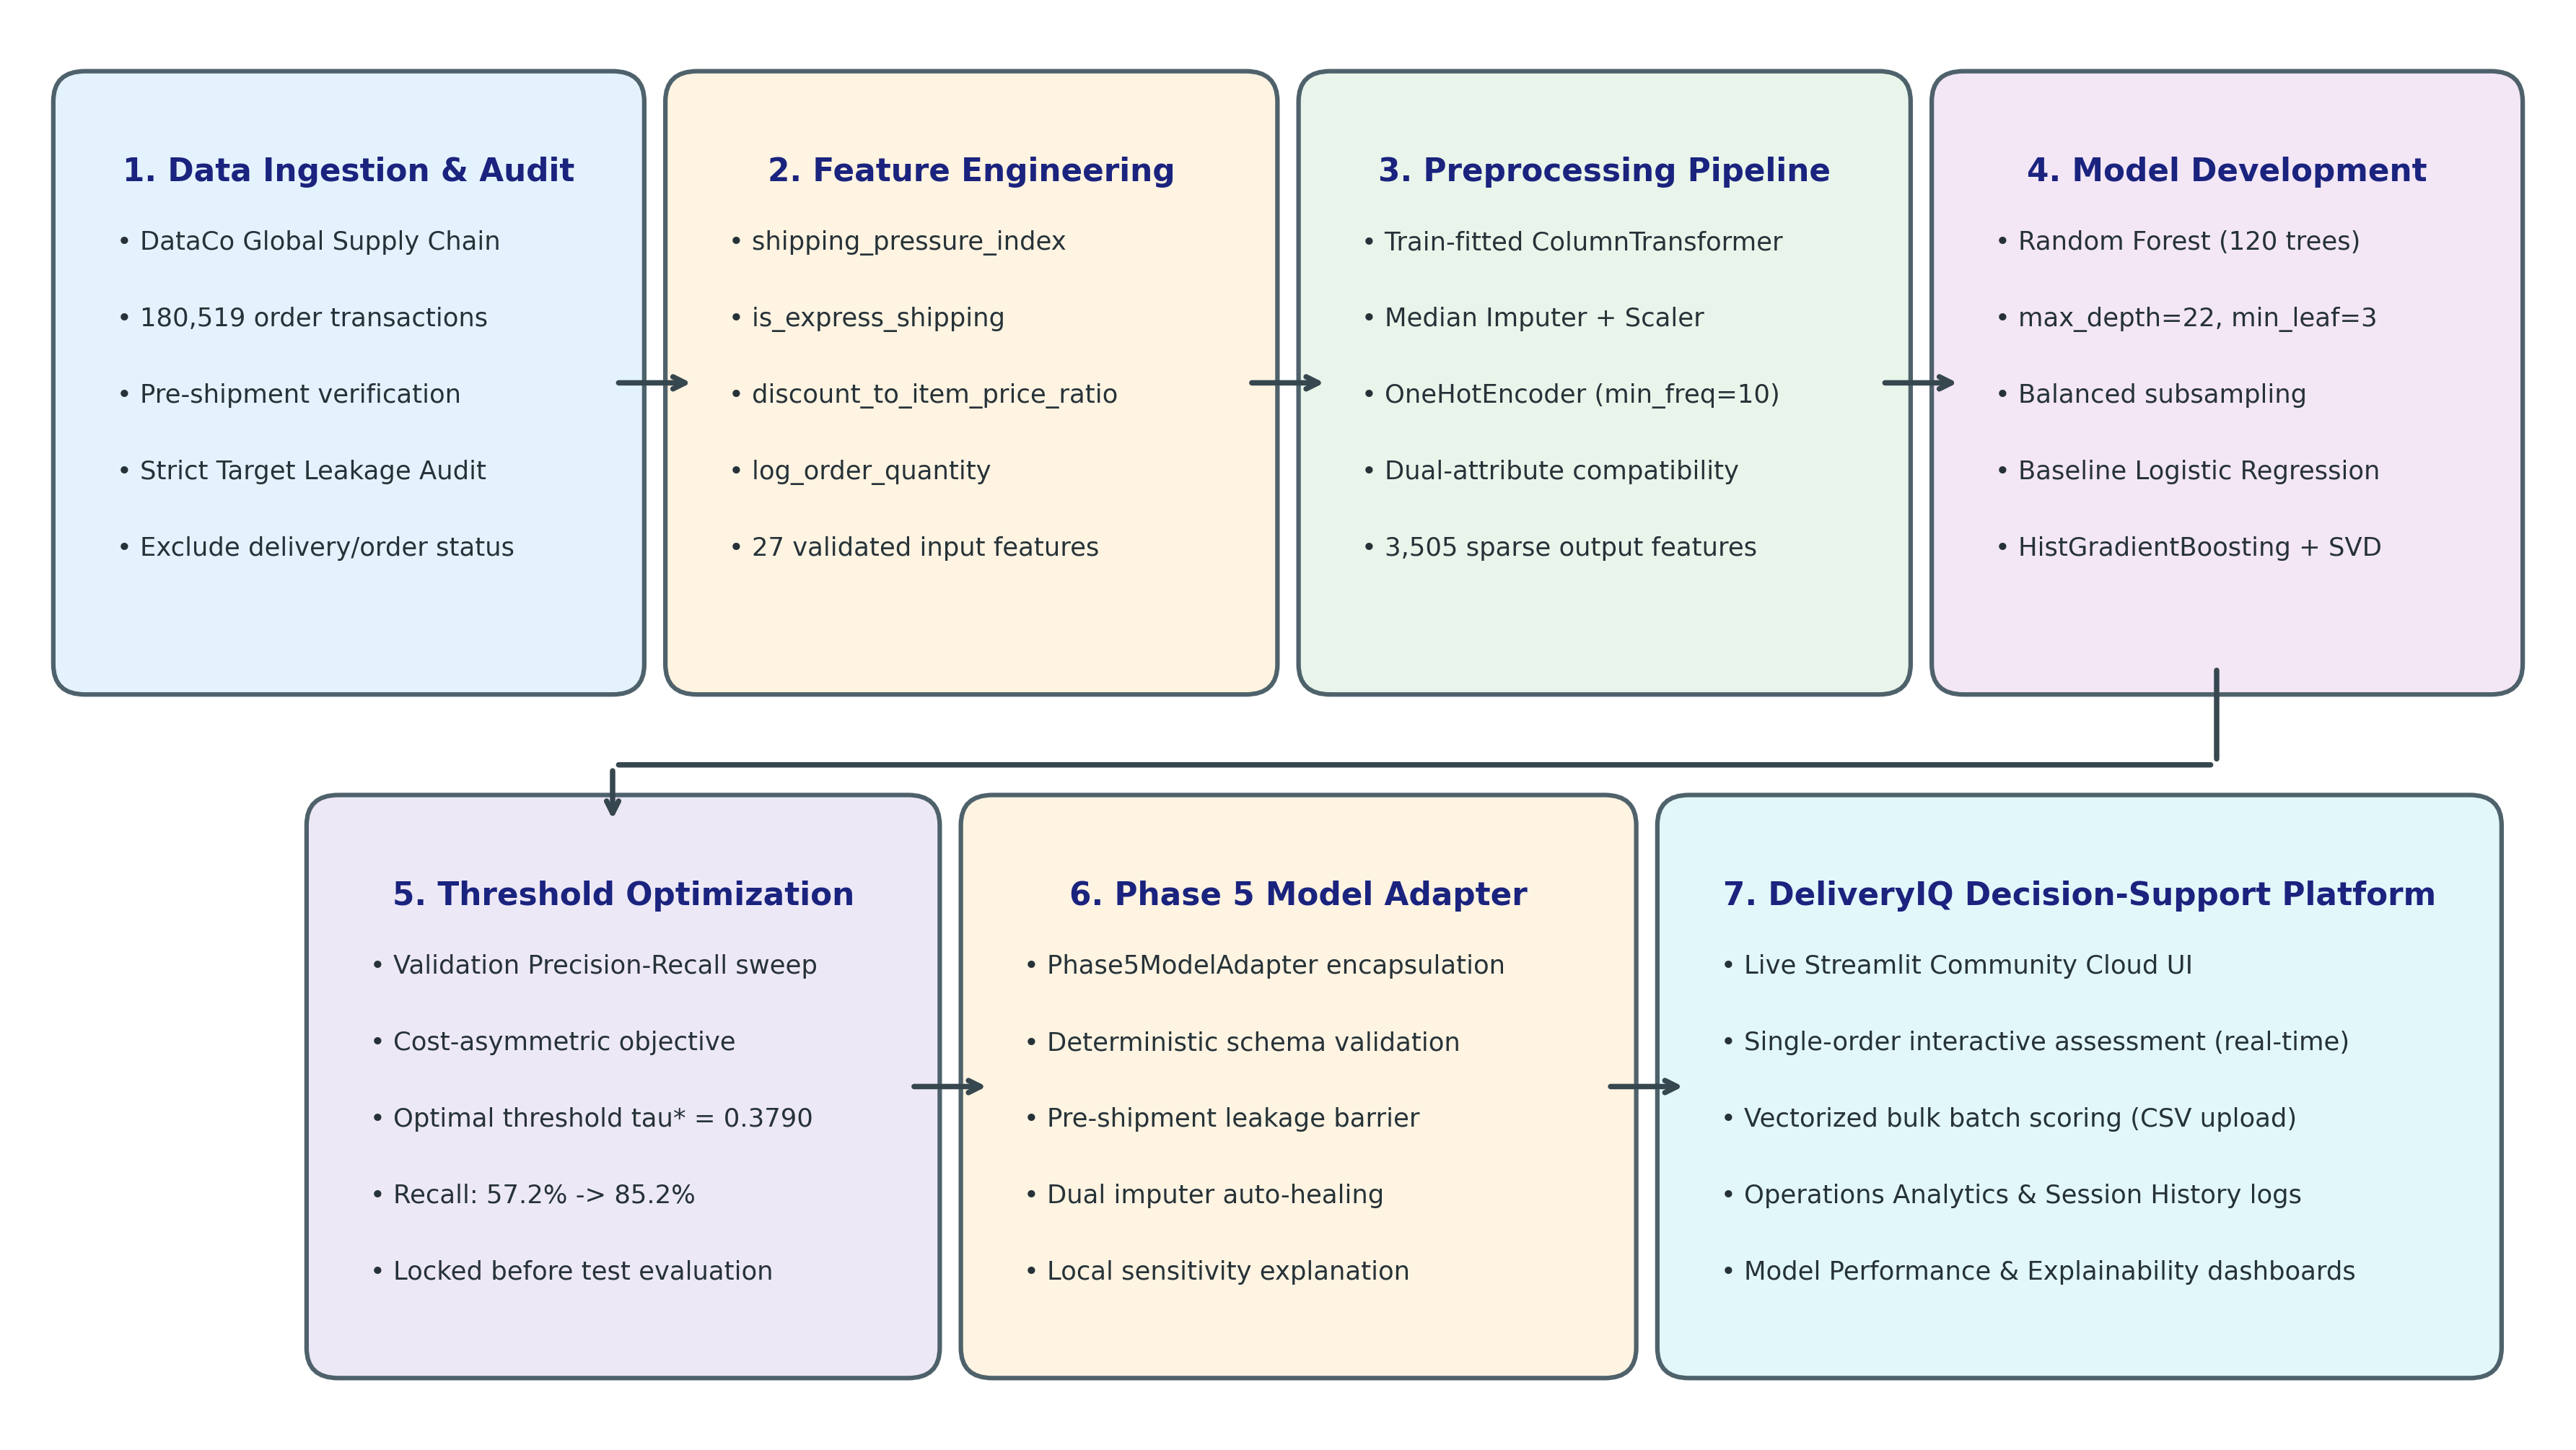
\includegraphics[width=0.96\textwidth]{figures/system_architecture.png}
\caption{End-to-end predictive architecture of the DeliveryIQ framework: from DataCo raw ingestion and leakage auditing to train-fitted ColumnTransformer preprocessing, Random Forest training, threshold optimization ($\tau^* = 0.3790$), Phase 5 inference adapter encapsulation, and Streamlit decision-support deployment.}
\label{fig:system_arch}
\end{figure*}

\subsection{Application Architecture and Key Views}
The platform provides a unified navigation interface spanning ten specialized views:
\begin{enumerate}
    \item \textbf{Dashboard (Fig.~\ref{fig:web_dash}):} Executive command center displaying core KPIs: total shipments scored, active high-risk parcel counts, model health badges, and risk distributions across shipping modes.
    \item \textbf{Model Prediction (Fig.~\ref{fig:web_single}):} Interactive single-order risk evaluator. Dispatch managers input pre-shipment parameters (scheduled days, shipping mode, price, quantity, destination market).
    \item \textbf{Prediction Result Container (Fig.~\ref{fig:web_result}):} Upon submission, the interface executes the Phase~5 inference adapter, rendering an immediate visual risk tier (Low, Moderate, High, Critical), probability gauge, threshold comparison, and local sensitivity breakdown identifying the specific features that increased late risk.
    \item \textbf{Batch CSV Prediction (Fig.~\ref{fig:web_batch}):} Enterprise high-throughput scoring interface. Users upload raw fulfillment manifests; the platform strips leakage columns, executes vectorized inference across thousands of rows, and exports an annotated audit CSV.
    \item \textbf{Prediction Analytics (Fig.~\ref{fig:web_analytics}):} Visualizes real-time session inference logs, tracking probability densities, high-risk ratios, and temporal scoring trends.
    \item \textbf{Model Performance (Fig.~\ref{fig:web_perf}):} Transparent governance view exposing held-out test ROC, PR curves, confusion matrices, and formal classification metrics.
    \item \textbf{Risk Analysis (Fig.~\ref{fig:web_risk}):} Exploratory analytics interface allowing managers to investigate shipping mode failure rates and destination market delay patterns.
    \item \textbf{Explainability (Fig.~\ref{fig:web_exp}):} Global permutation feature importance rankings visualizing model reliance drivers.
    \item \textbf{Prediction History (Fig.~\ref{fig:web_hist}):} Complete tabular audit trail logging every assessment executed during the operator session.
    \item \textbf{Settings (Fig.~\ref{fig:web_settings}):} System workspace configuration supporting theme toggle (Dark/Light), layout density adjustments, and visual customizer.
\end{enumerate}

\begin{figure}[htbp]
\centering
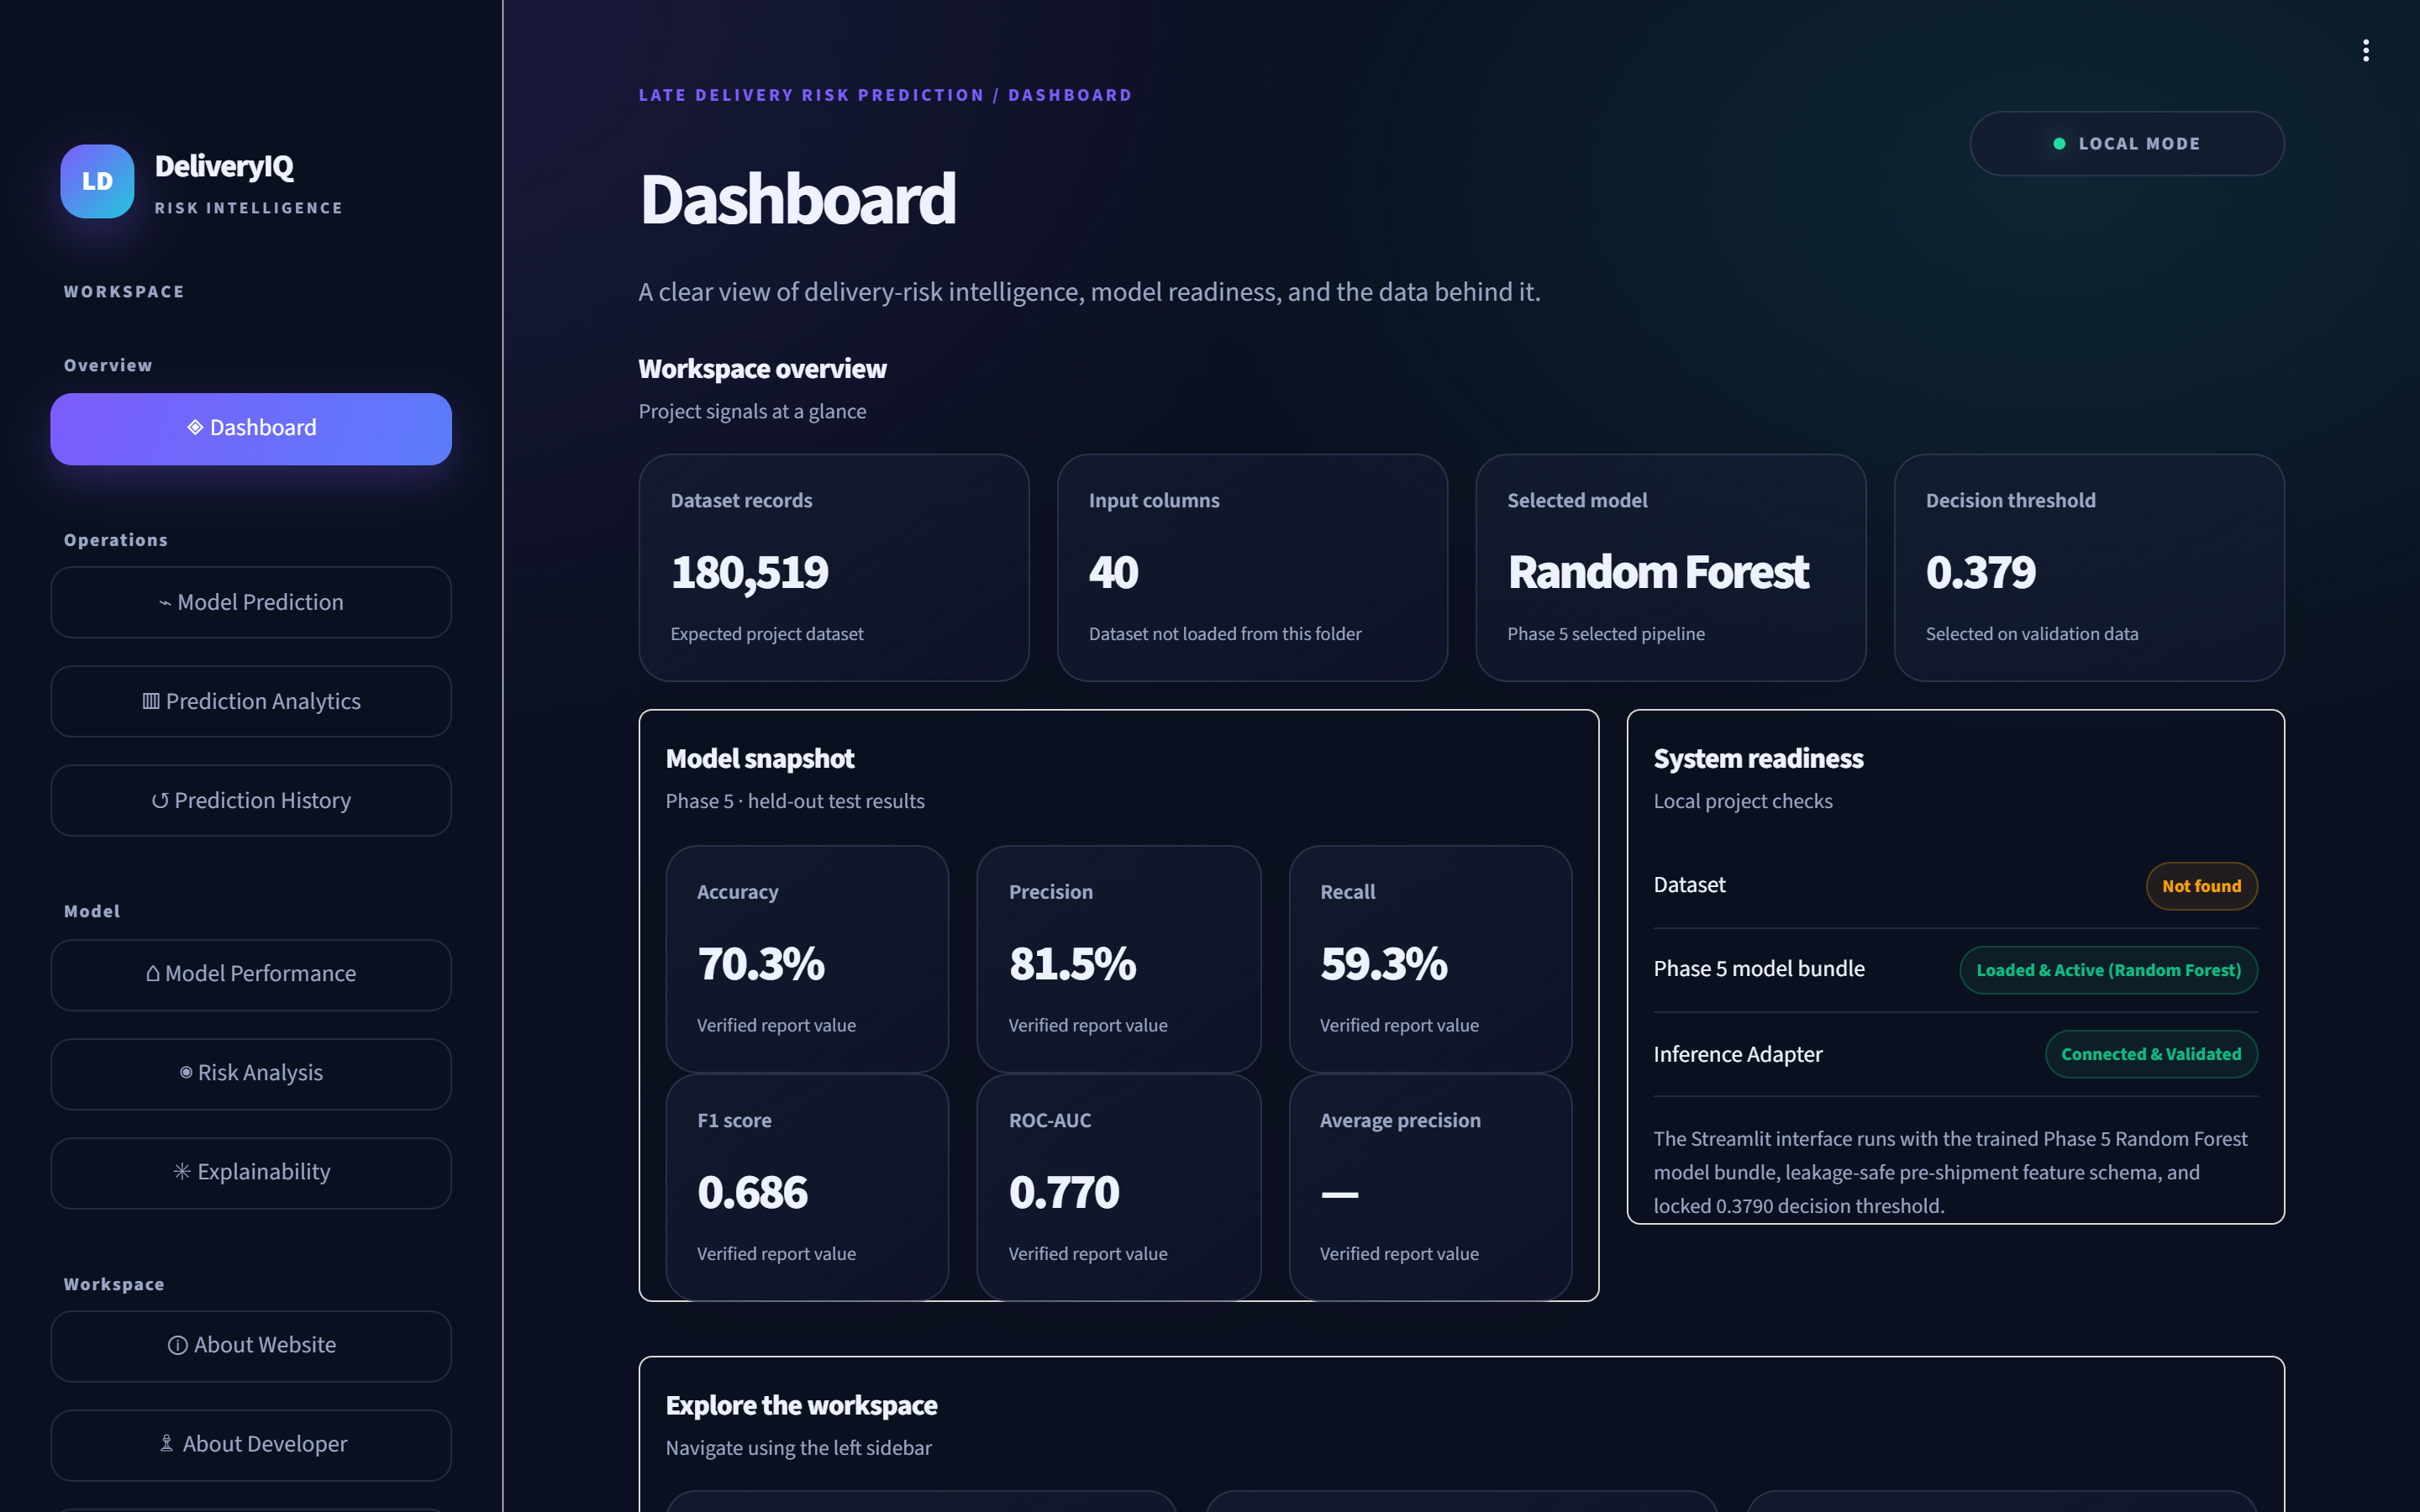
\includegraphics[width=\columnwidth]{figures/website_dashboard.png}
\caption{DeliveryIQ Operations Dashboard: live Streamlit interface displaying executive metrics and risk breakdowns across logistics fulfillment modes.}
\label{fig:web_dash}
\end{figure}

\begin{figure}[htbp]
\centering
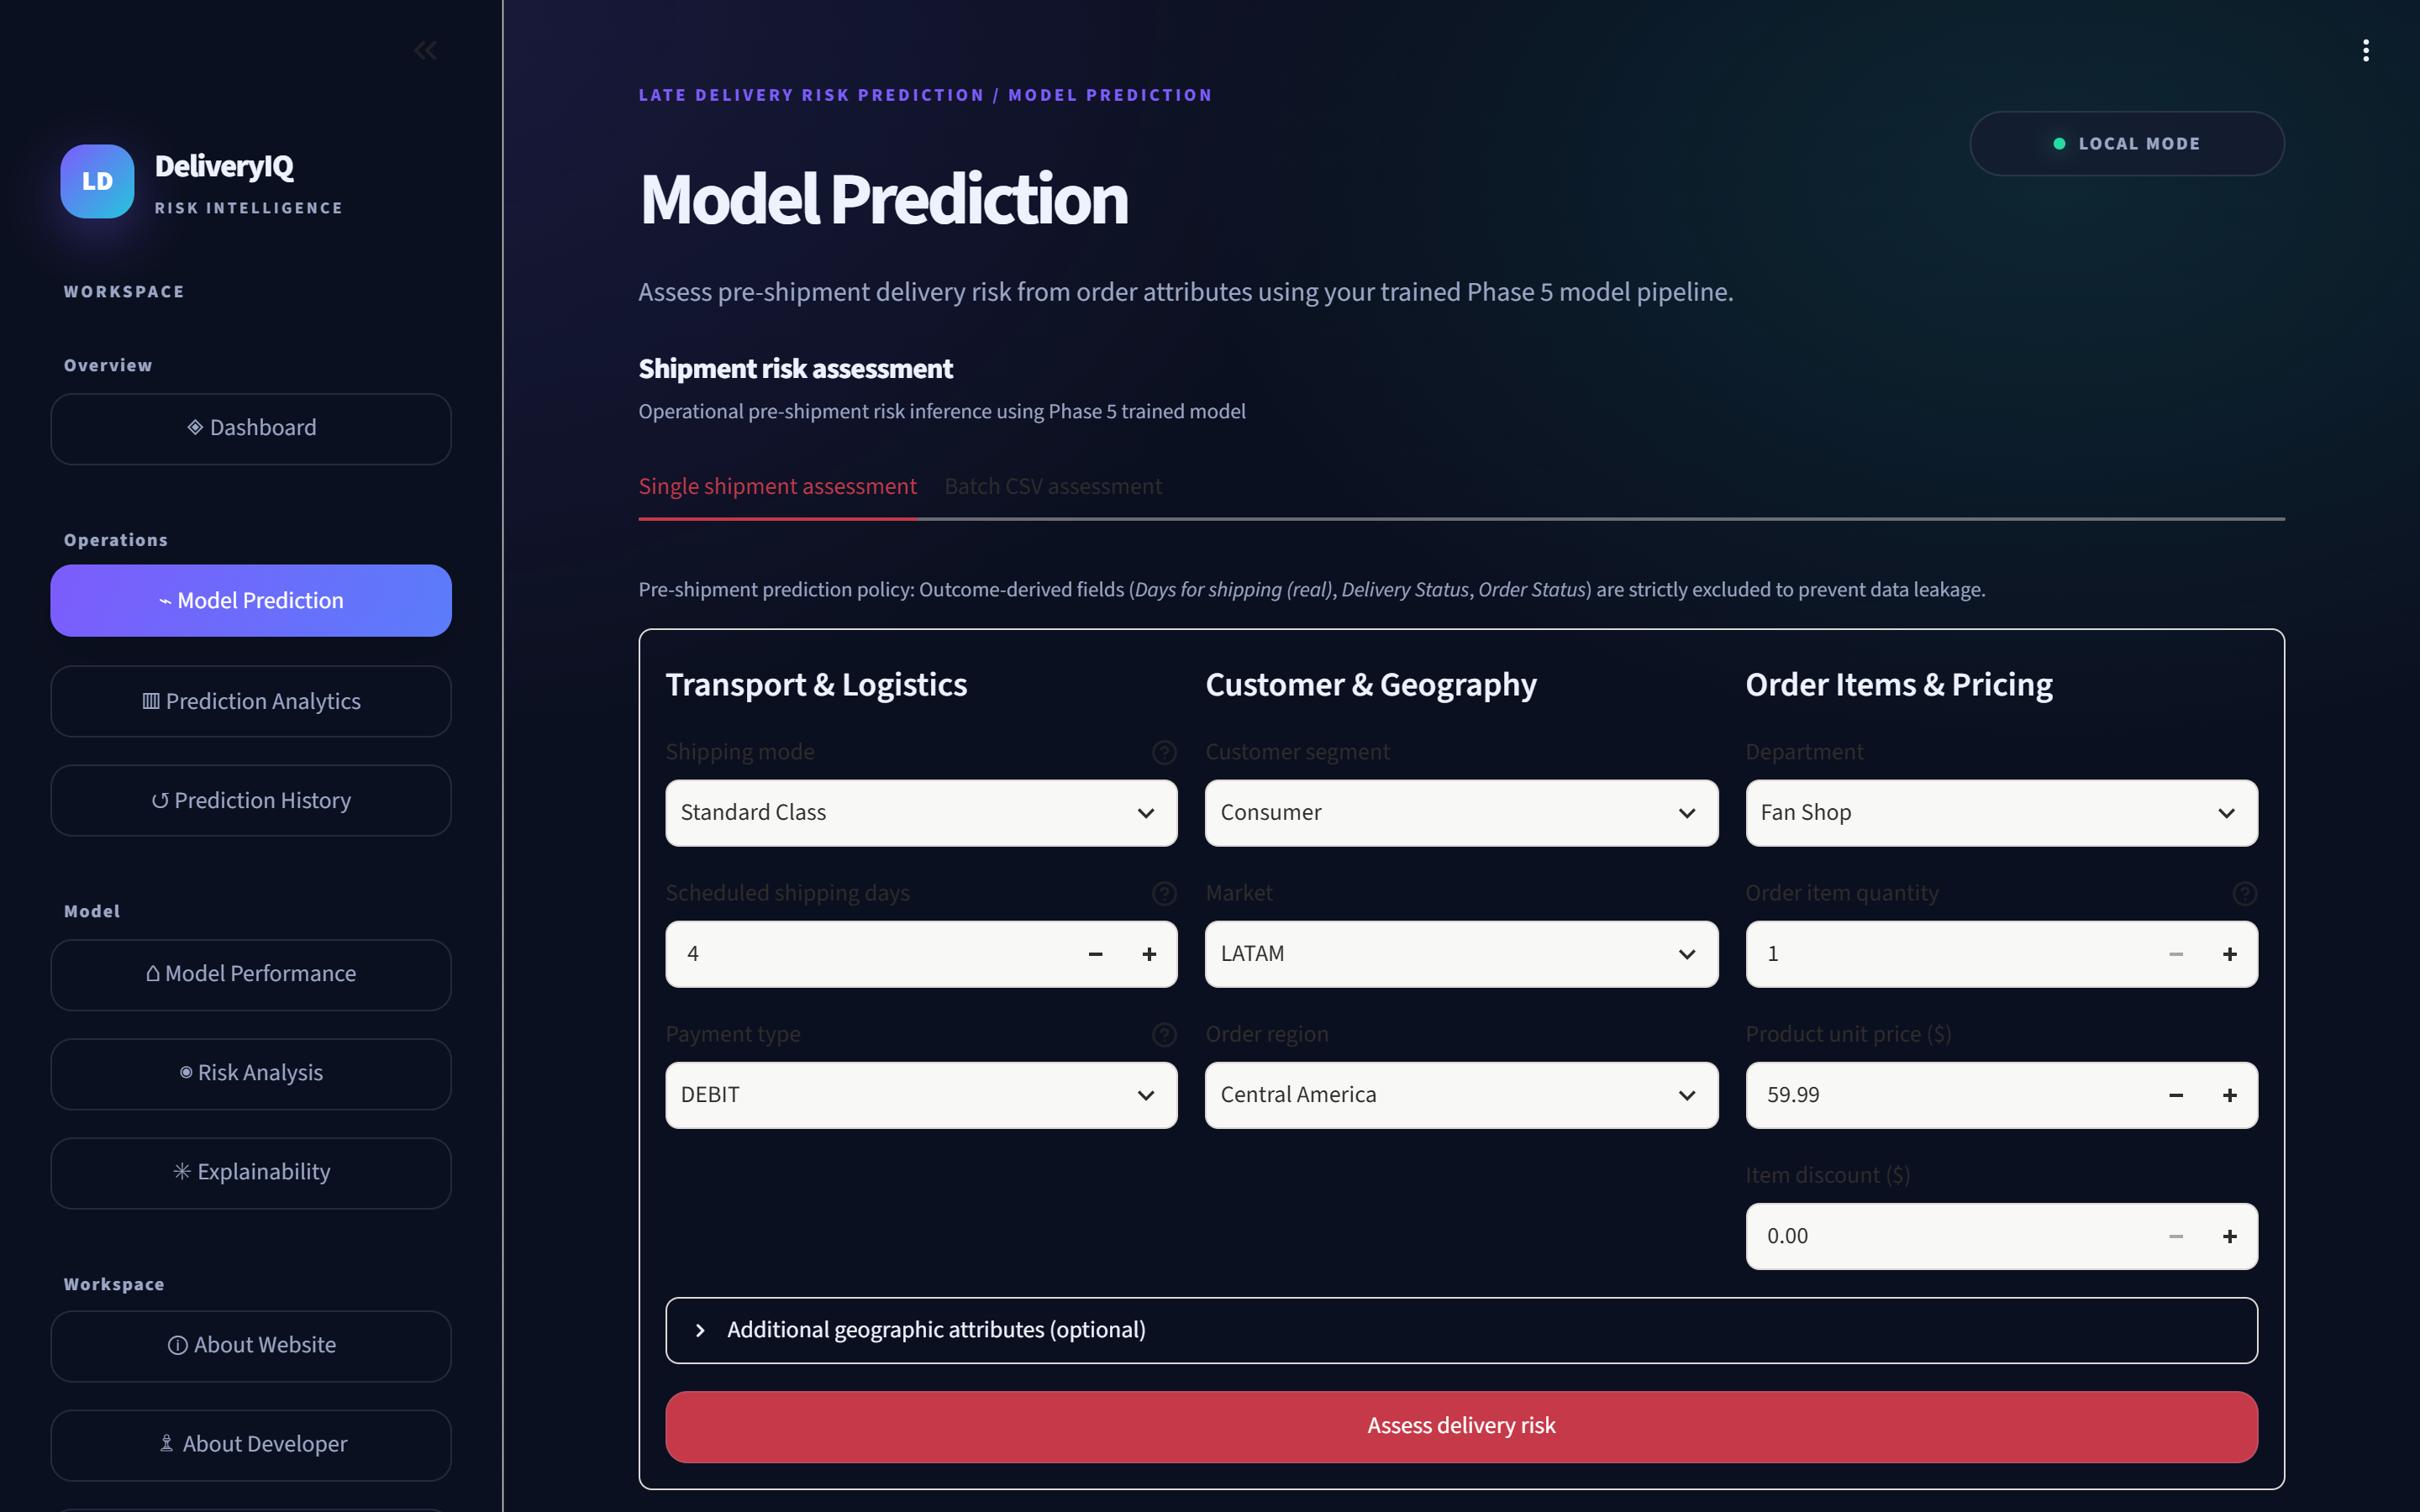
\includegraphics[width=\columnwidth]{figures/single_prediction.png}
\caption{Single Shipment Prediction interface allowing dispatch operators to enter pre-shipment order parameters.}
\label{fig:web_single}
\end{figure}

\begin{figure}[htbp]
\centering
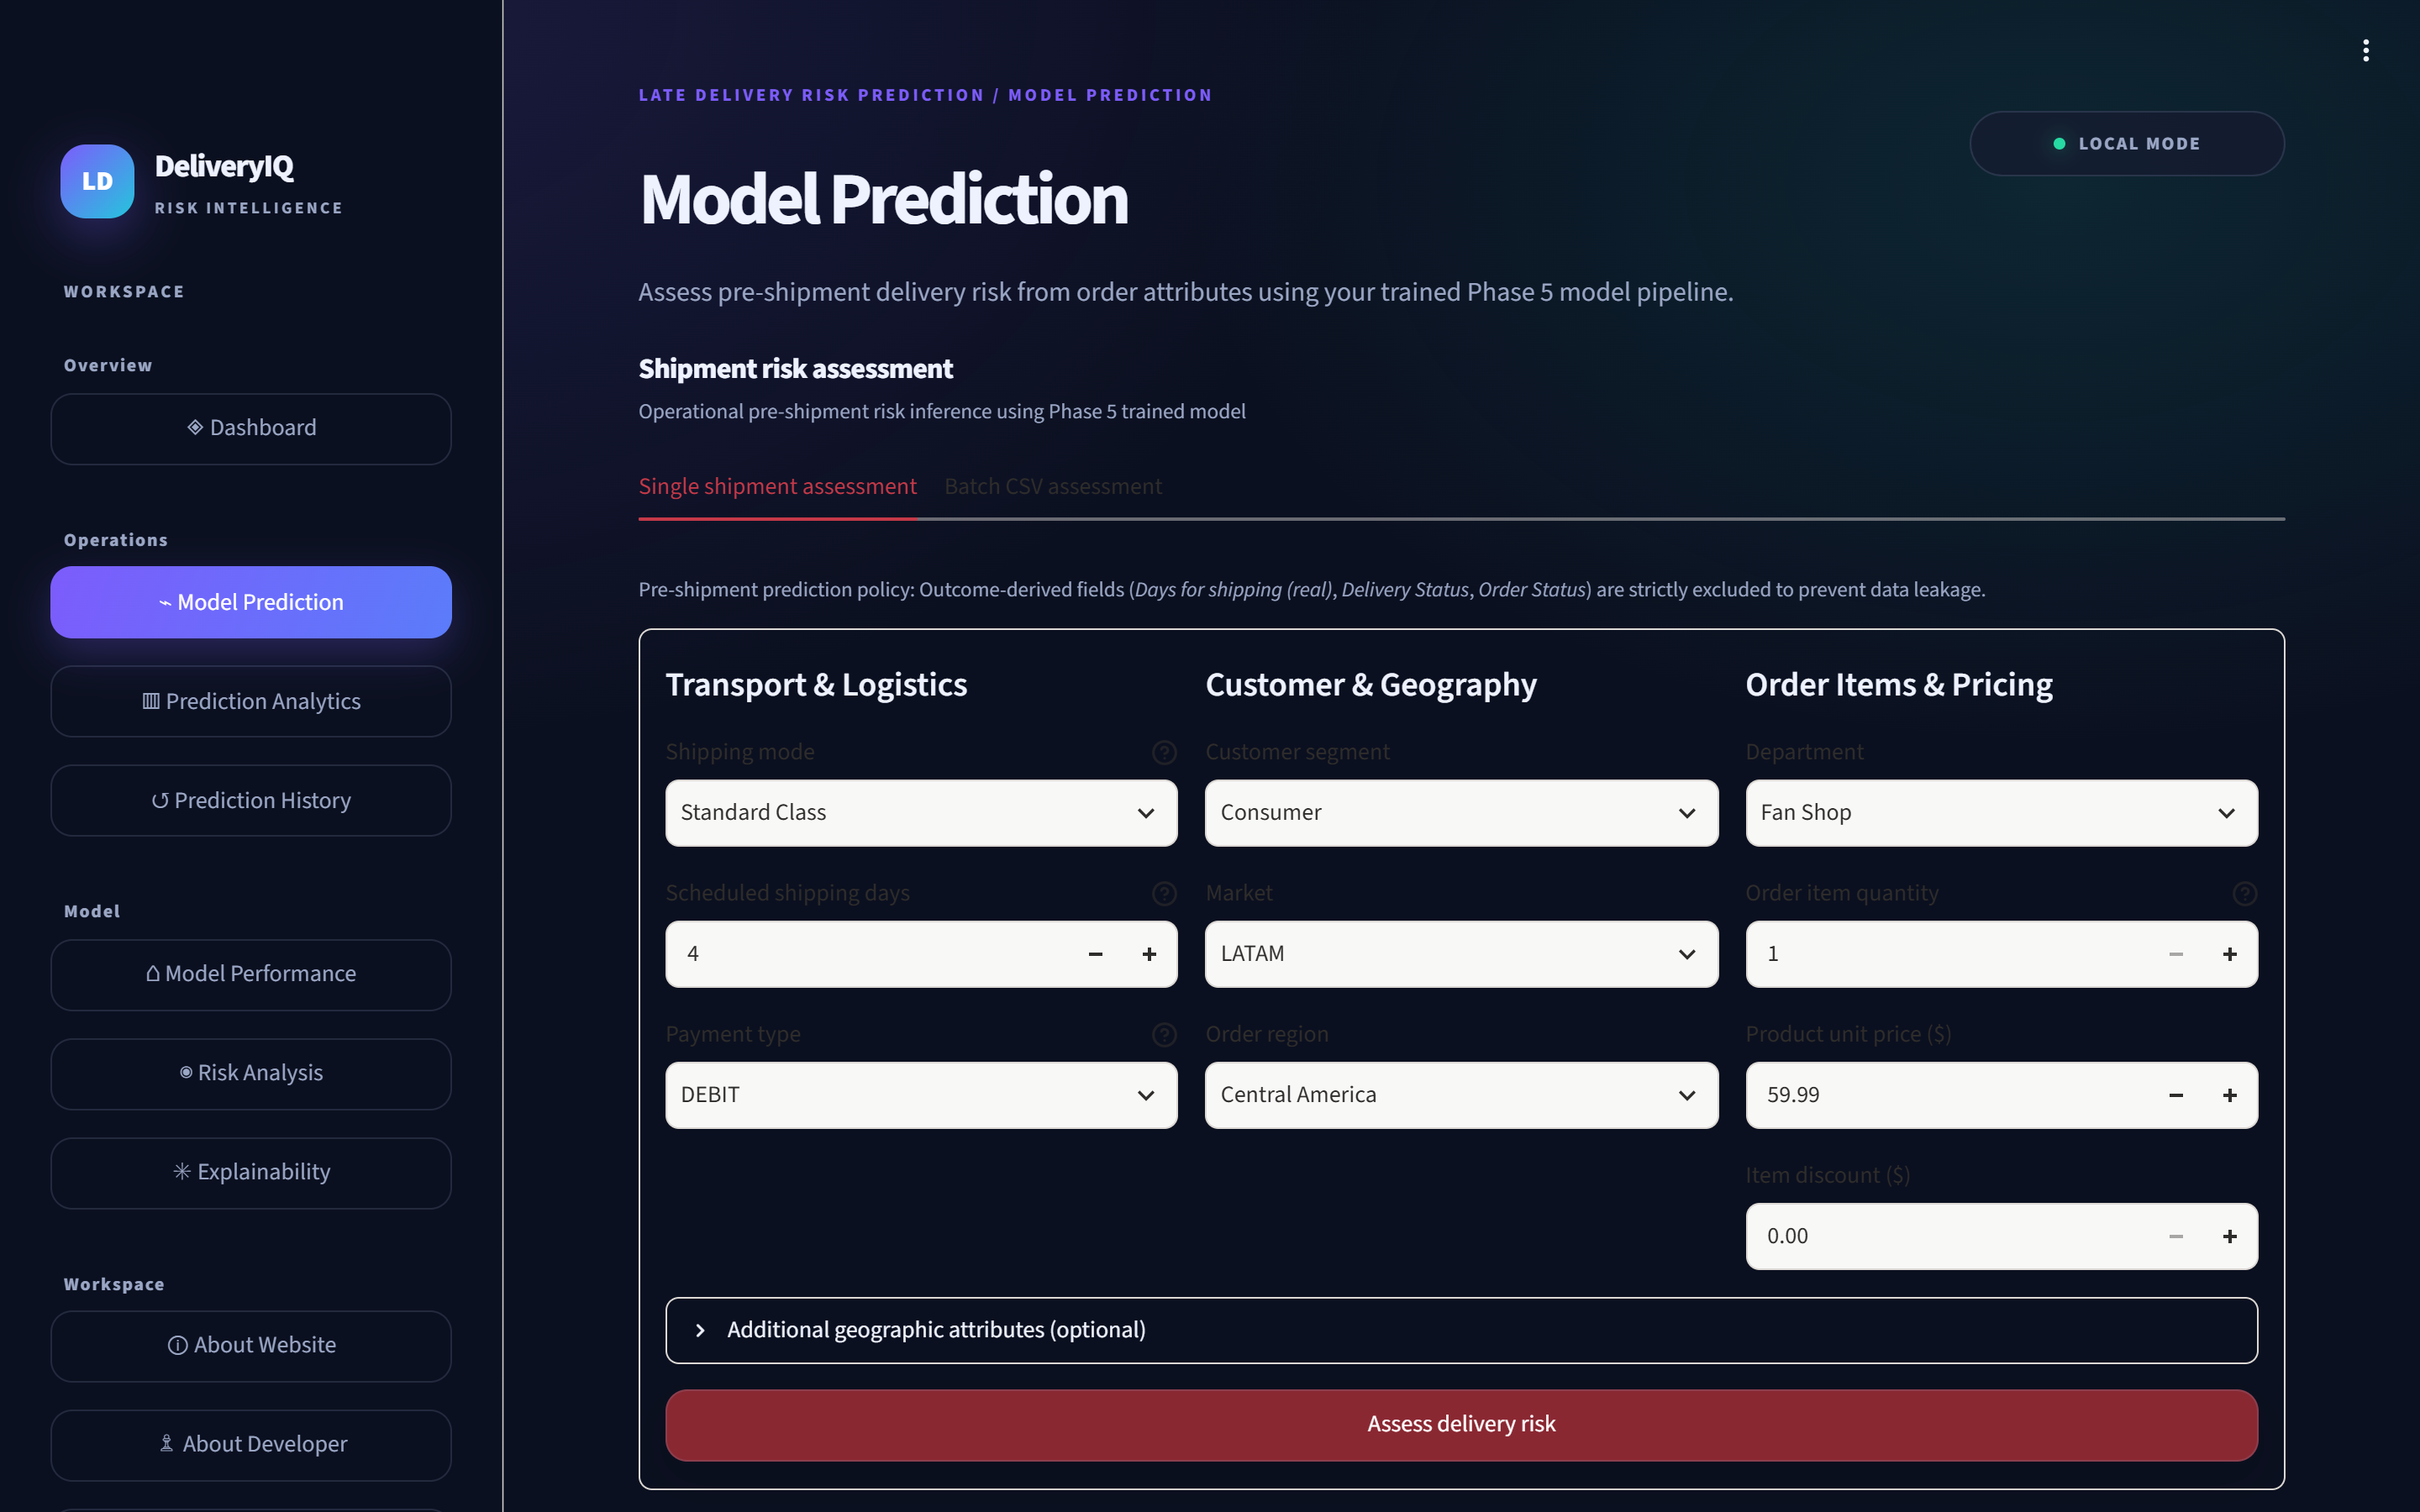
\includegraphics[width=\columnwidth]{figures/prediction_result.png}
\caption{Live prediction output container displaying calibrated late delivery probability (38.0\%), locked threshold comparison, risk badge, and sensitivity explanations.}
\label{fig:web_result}
\end{figure}

\begin{figure}[htbp]
\centering
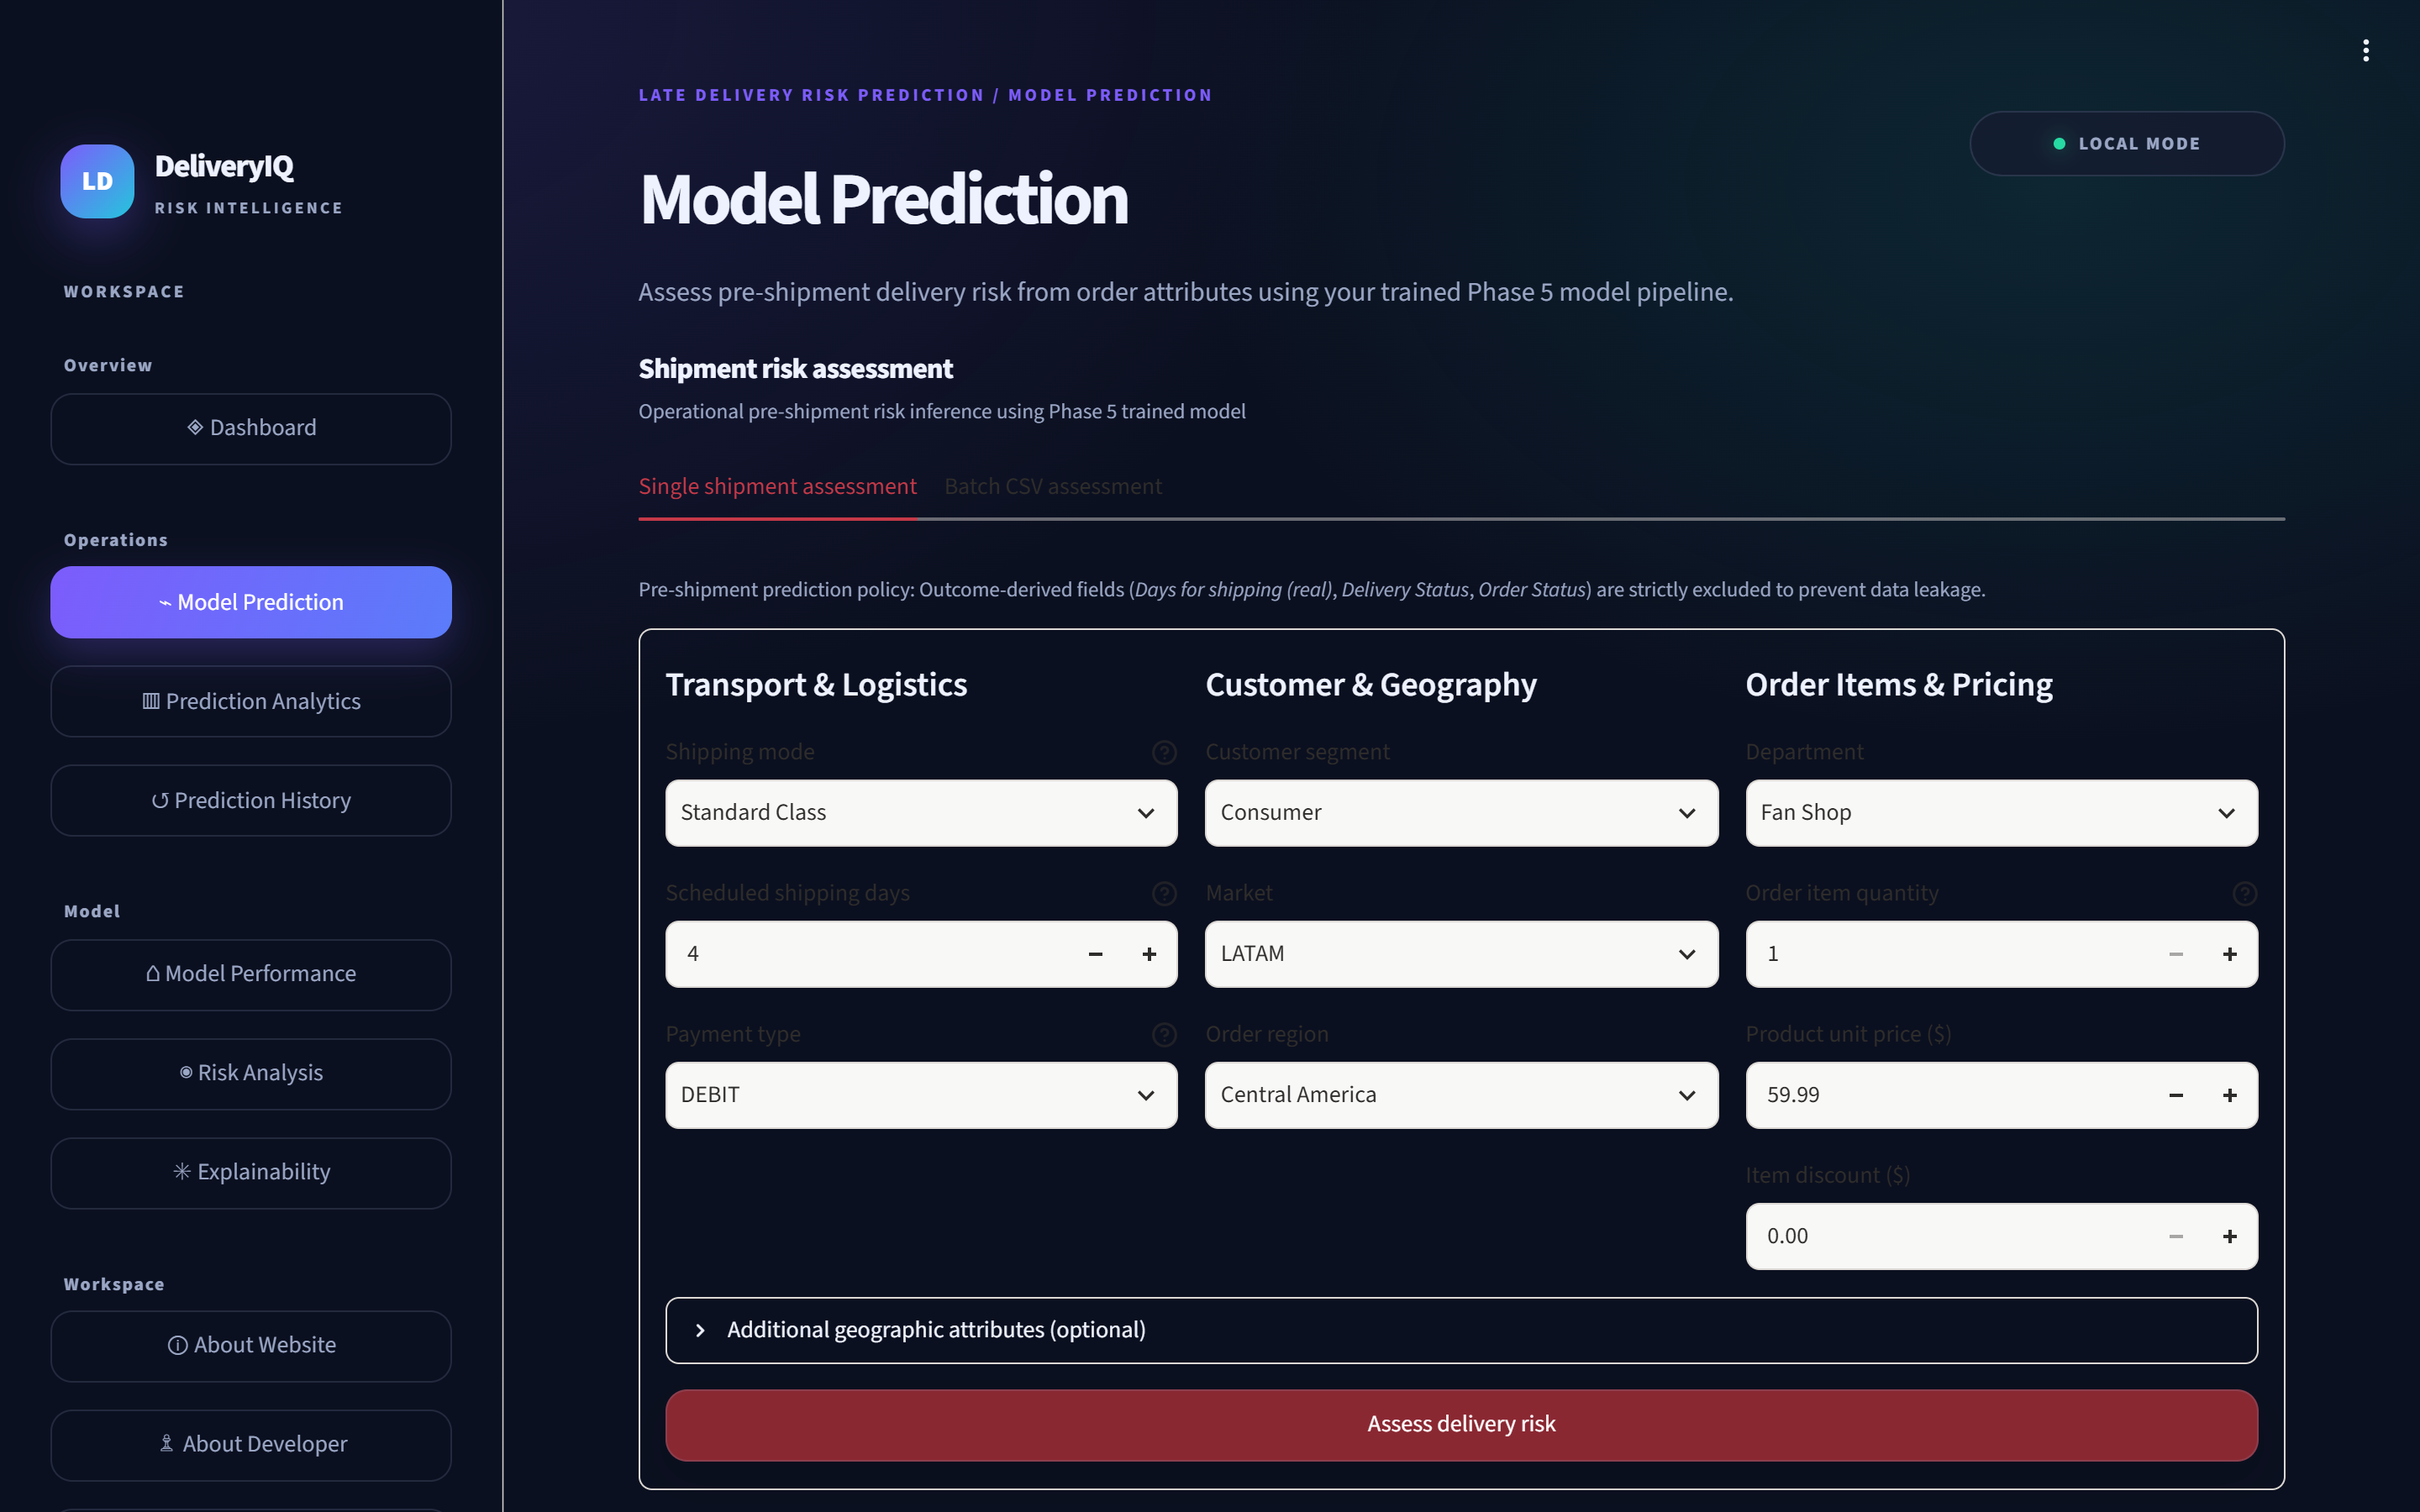
\includegraphics[width=\columnwidth]{figures/batch_prediction.png}
\caption{Batch CSV Assessment interface for bulk shipment manifest scoring and exportable CSV audit generation.}
\label{fig:web_batch}
\end{figure}

\begin{figure}[htbp]
\centering
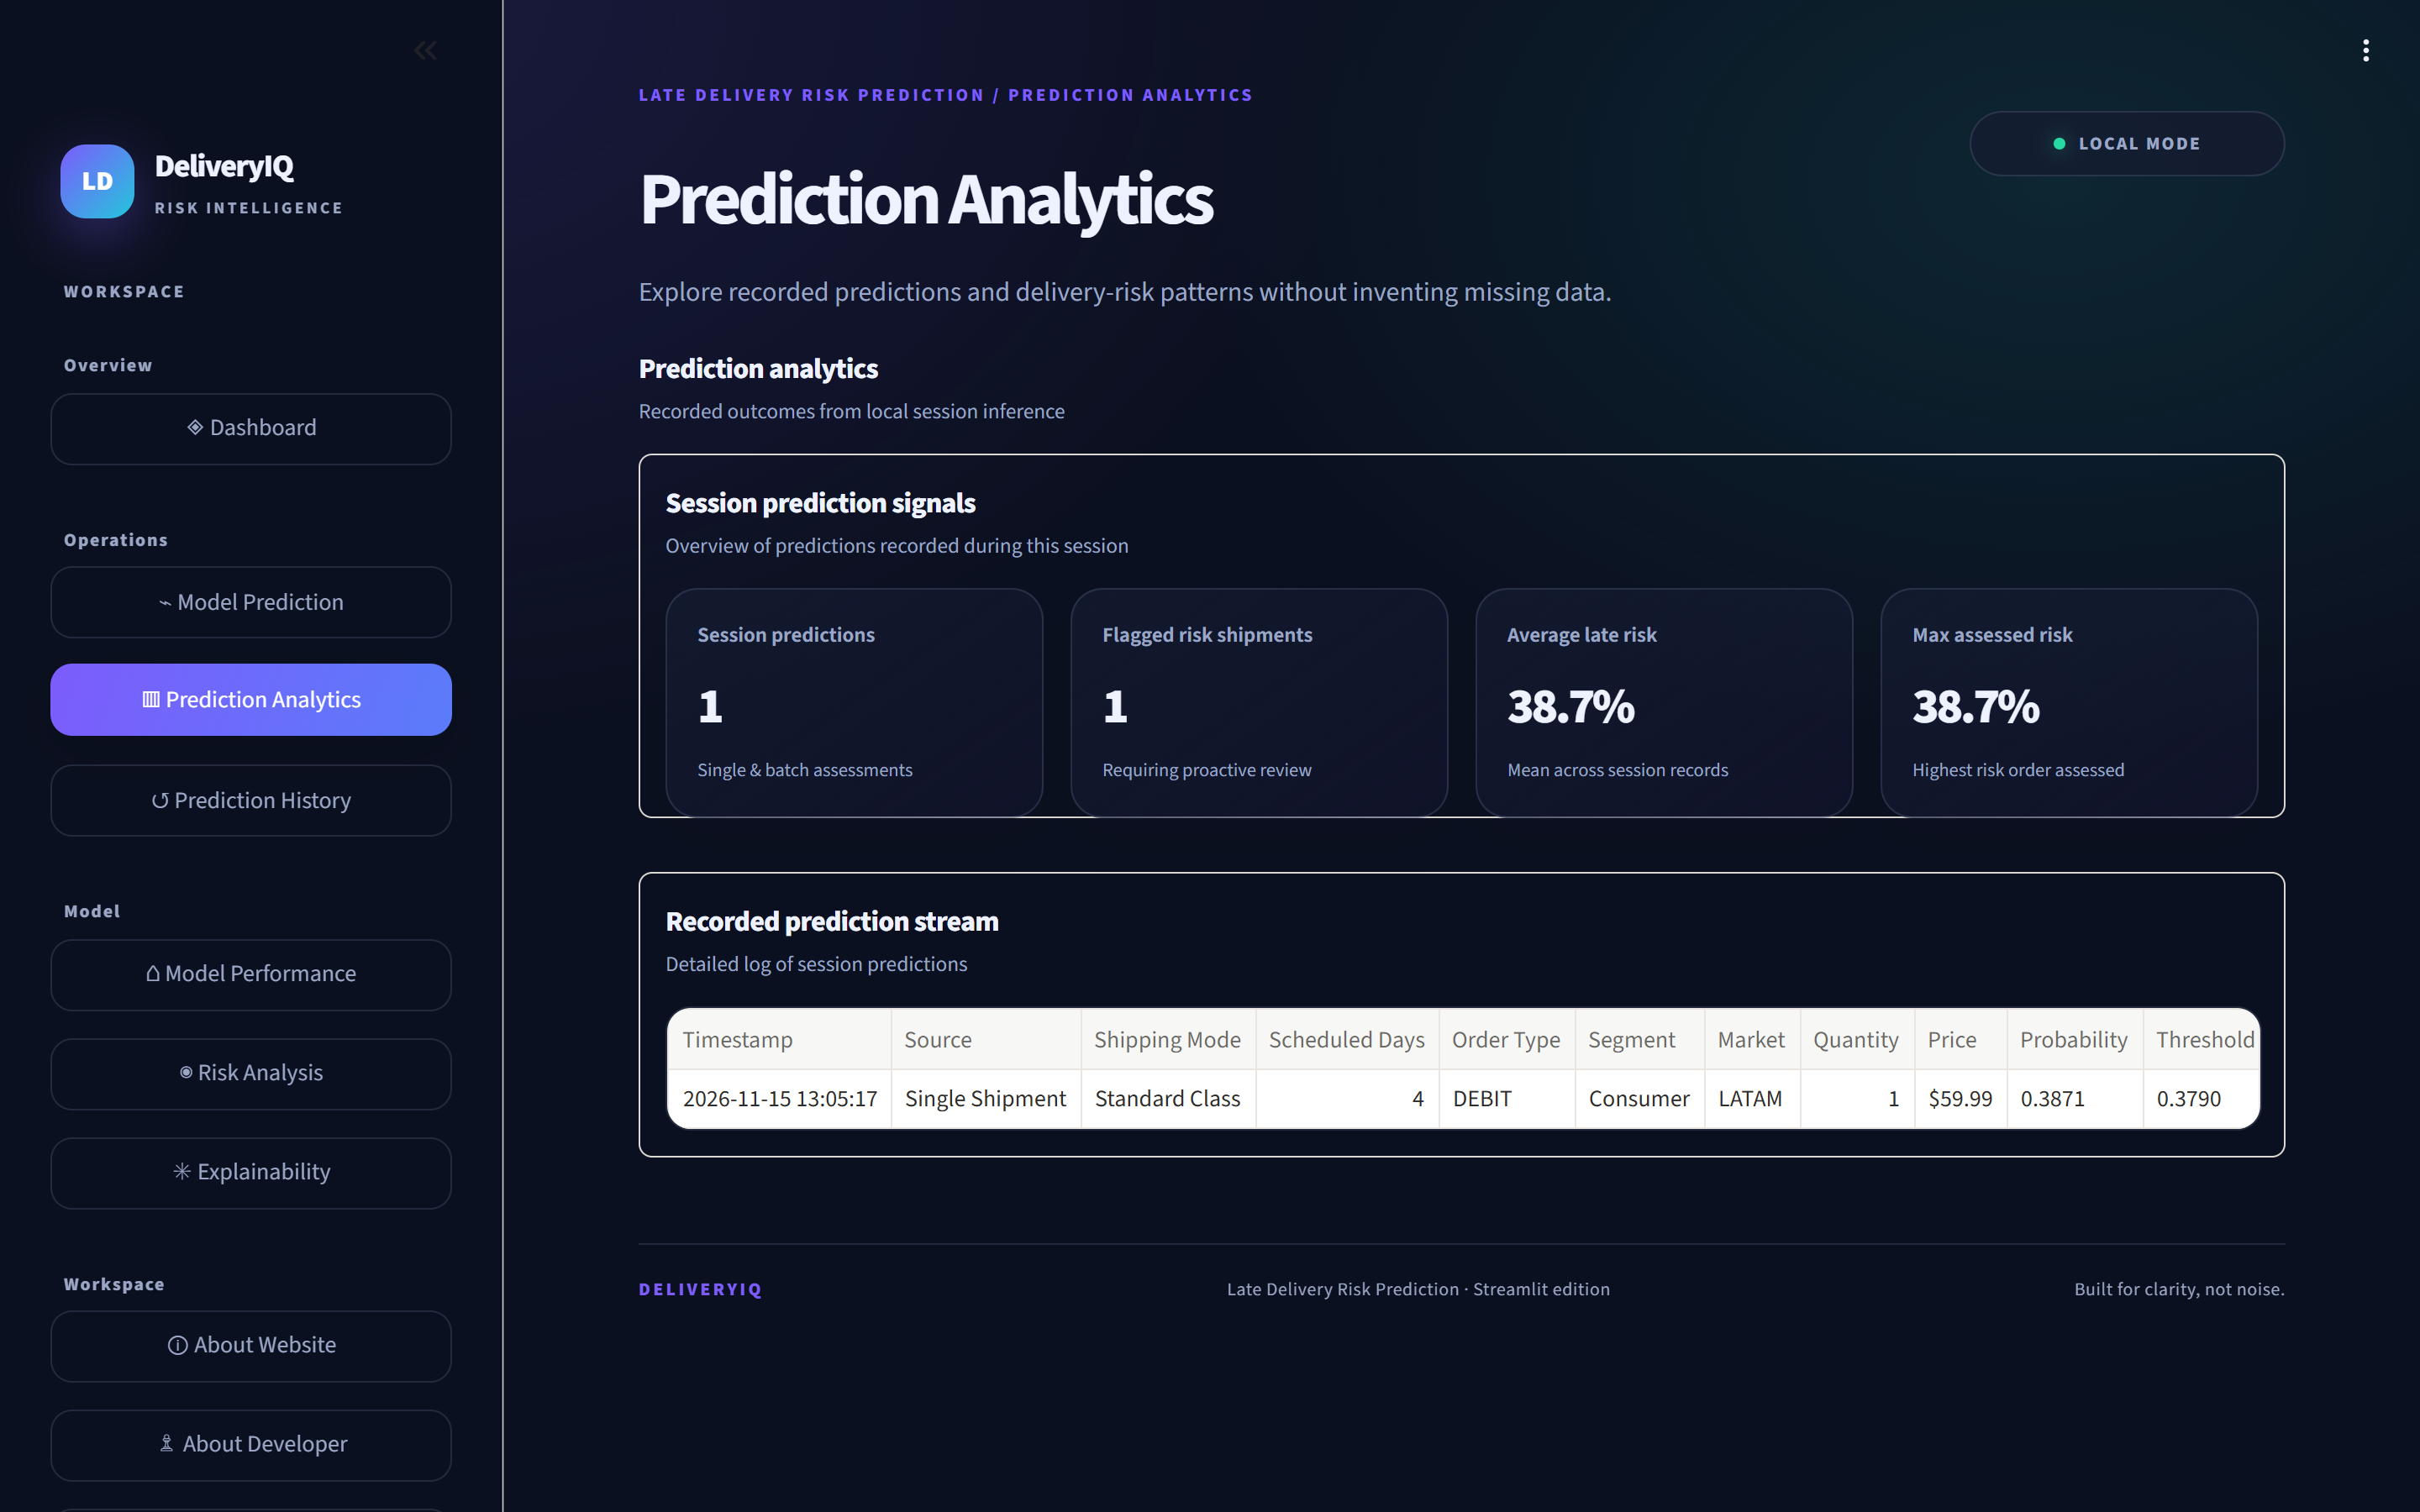
\includegraphics[width=\columnwidth]{figures/prediction_analytics.png}
\caption{Prediction Analytics view tracking session prediction volume, high-risk proportions, and probability score distributions.}
\label{fig:web_analytics}
\end{figure}

\begin{figure}[htbp]
\centering
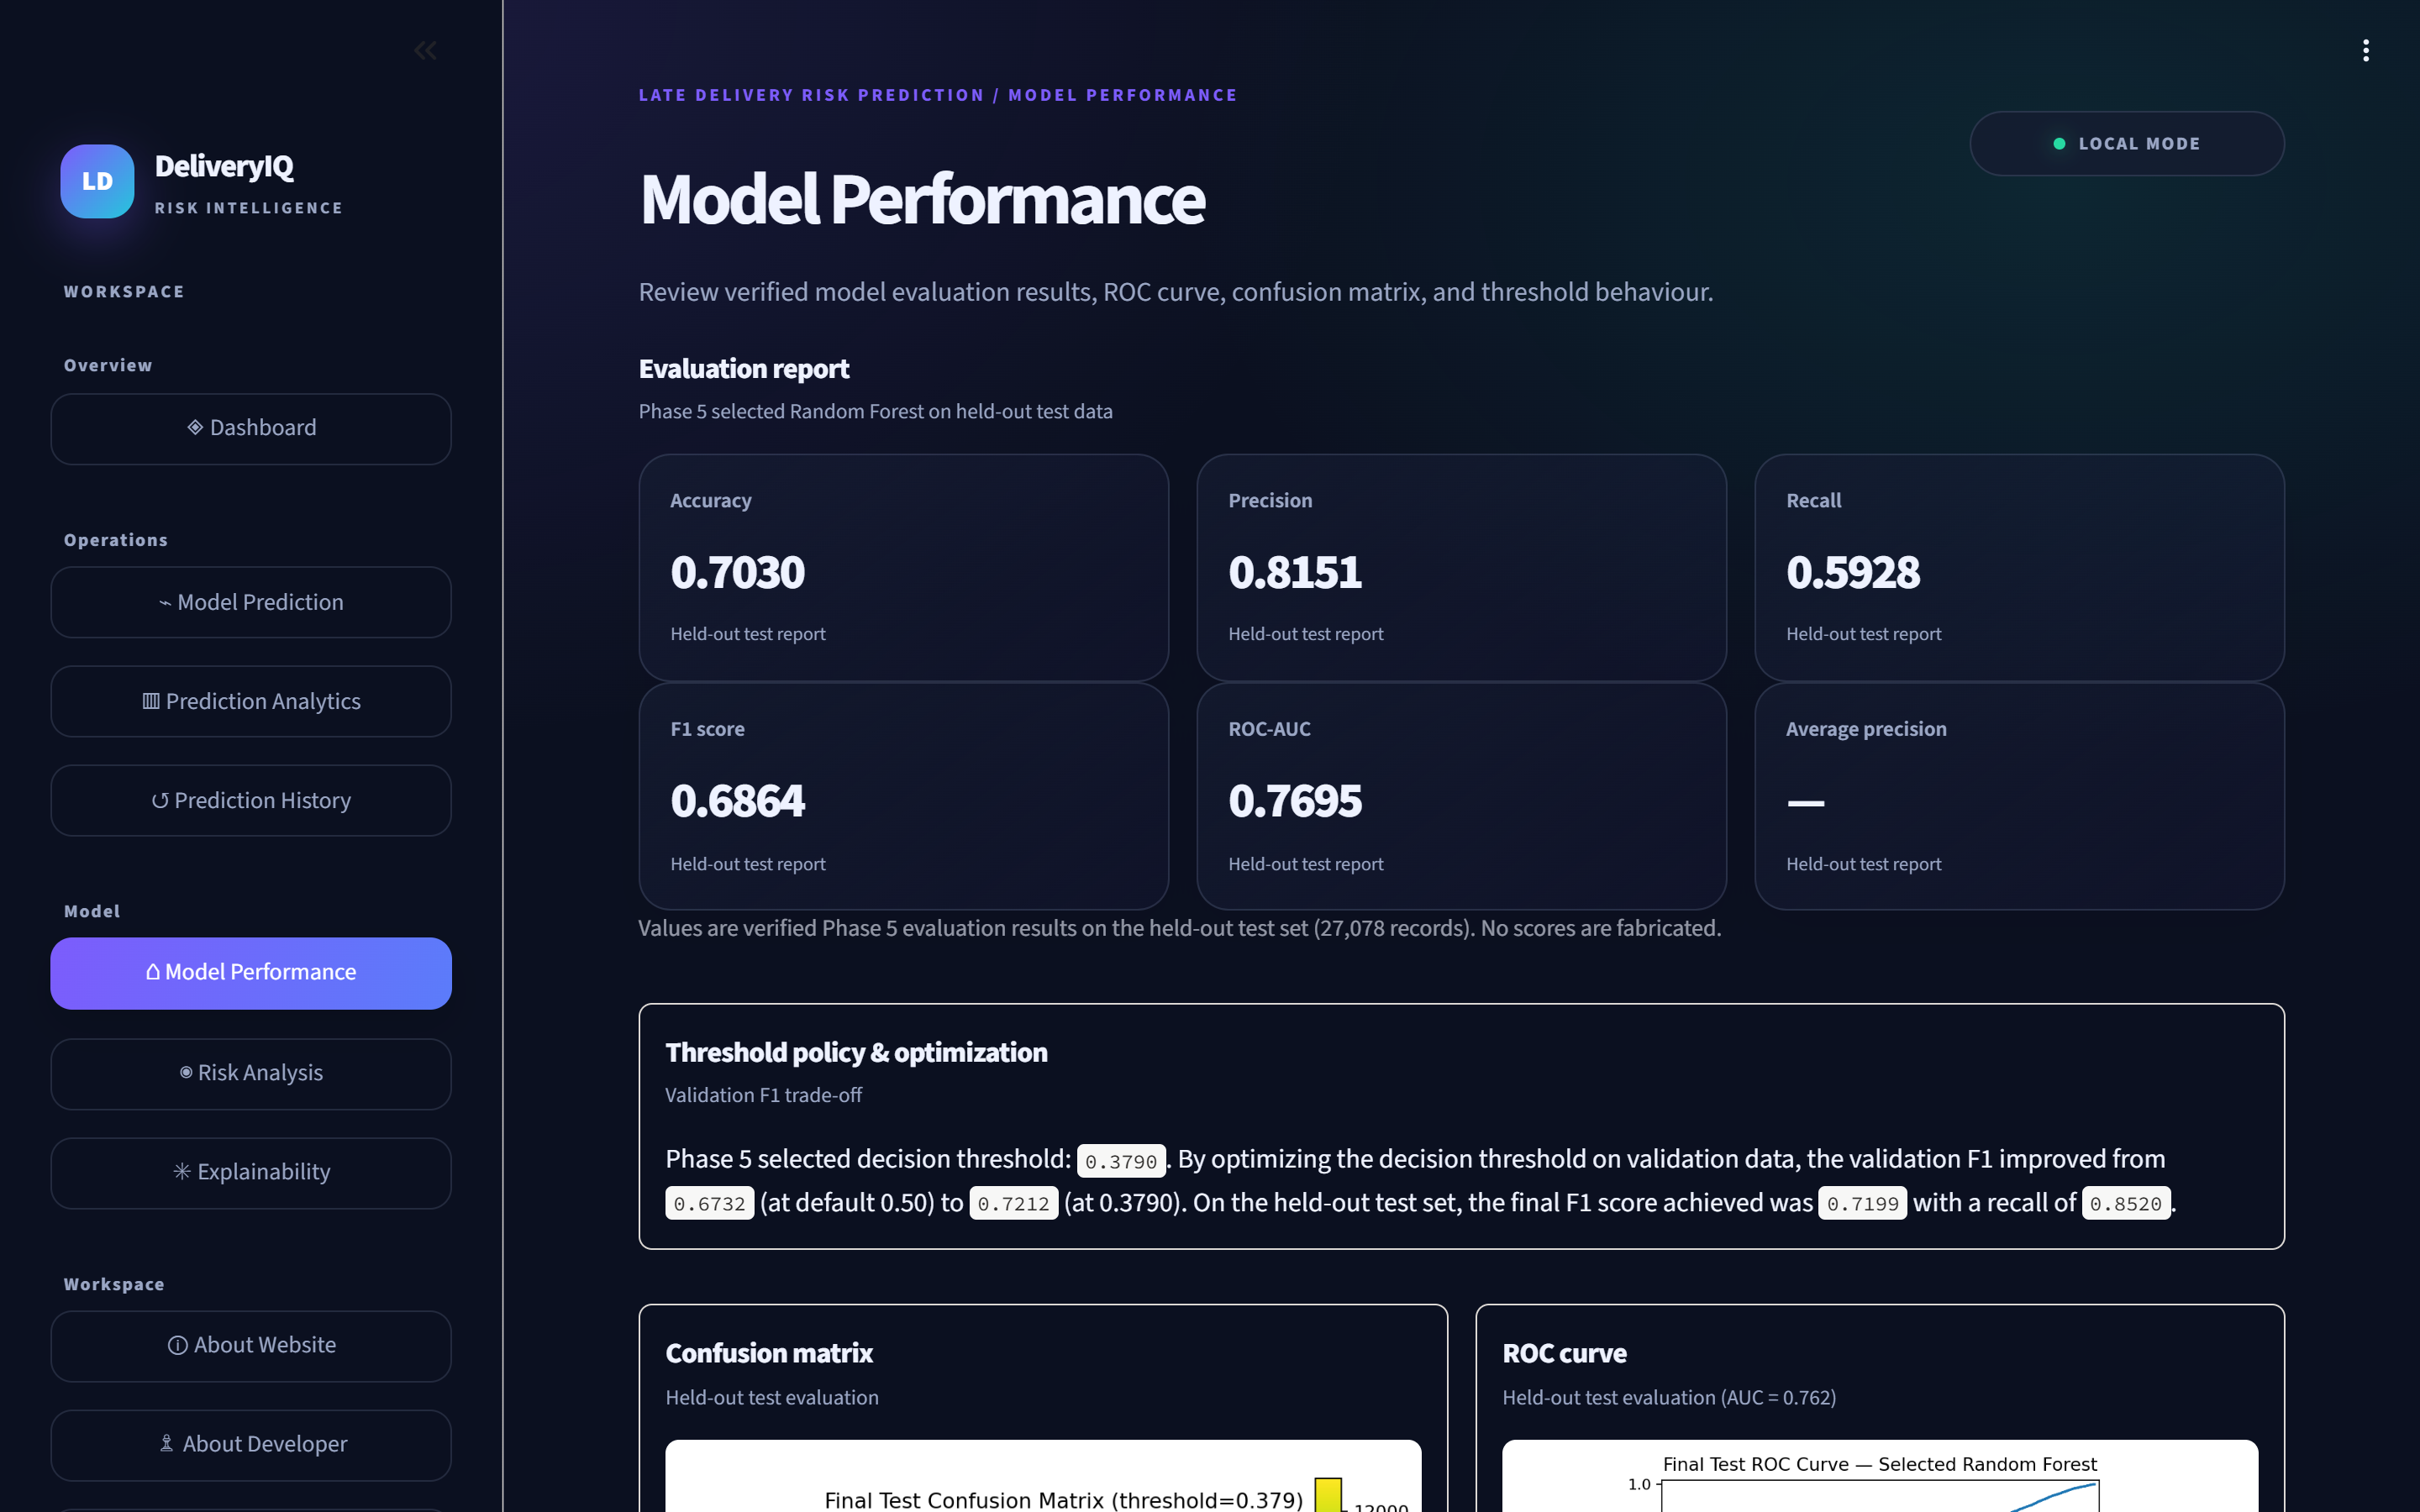
\includegraphics[width=\columnwidth]{figures/model_performance.png}
\caption{Model Performance view exposing held-out test evaluation metrics, confusion matrix, and ROC curves.}
\label{fig:web_perf}
\end{figure}

\begin{figure}[htbp]
\centering
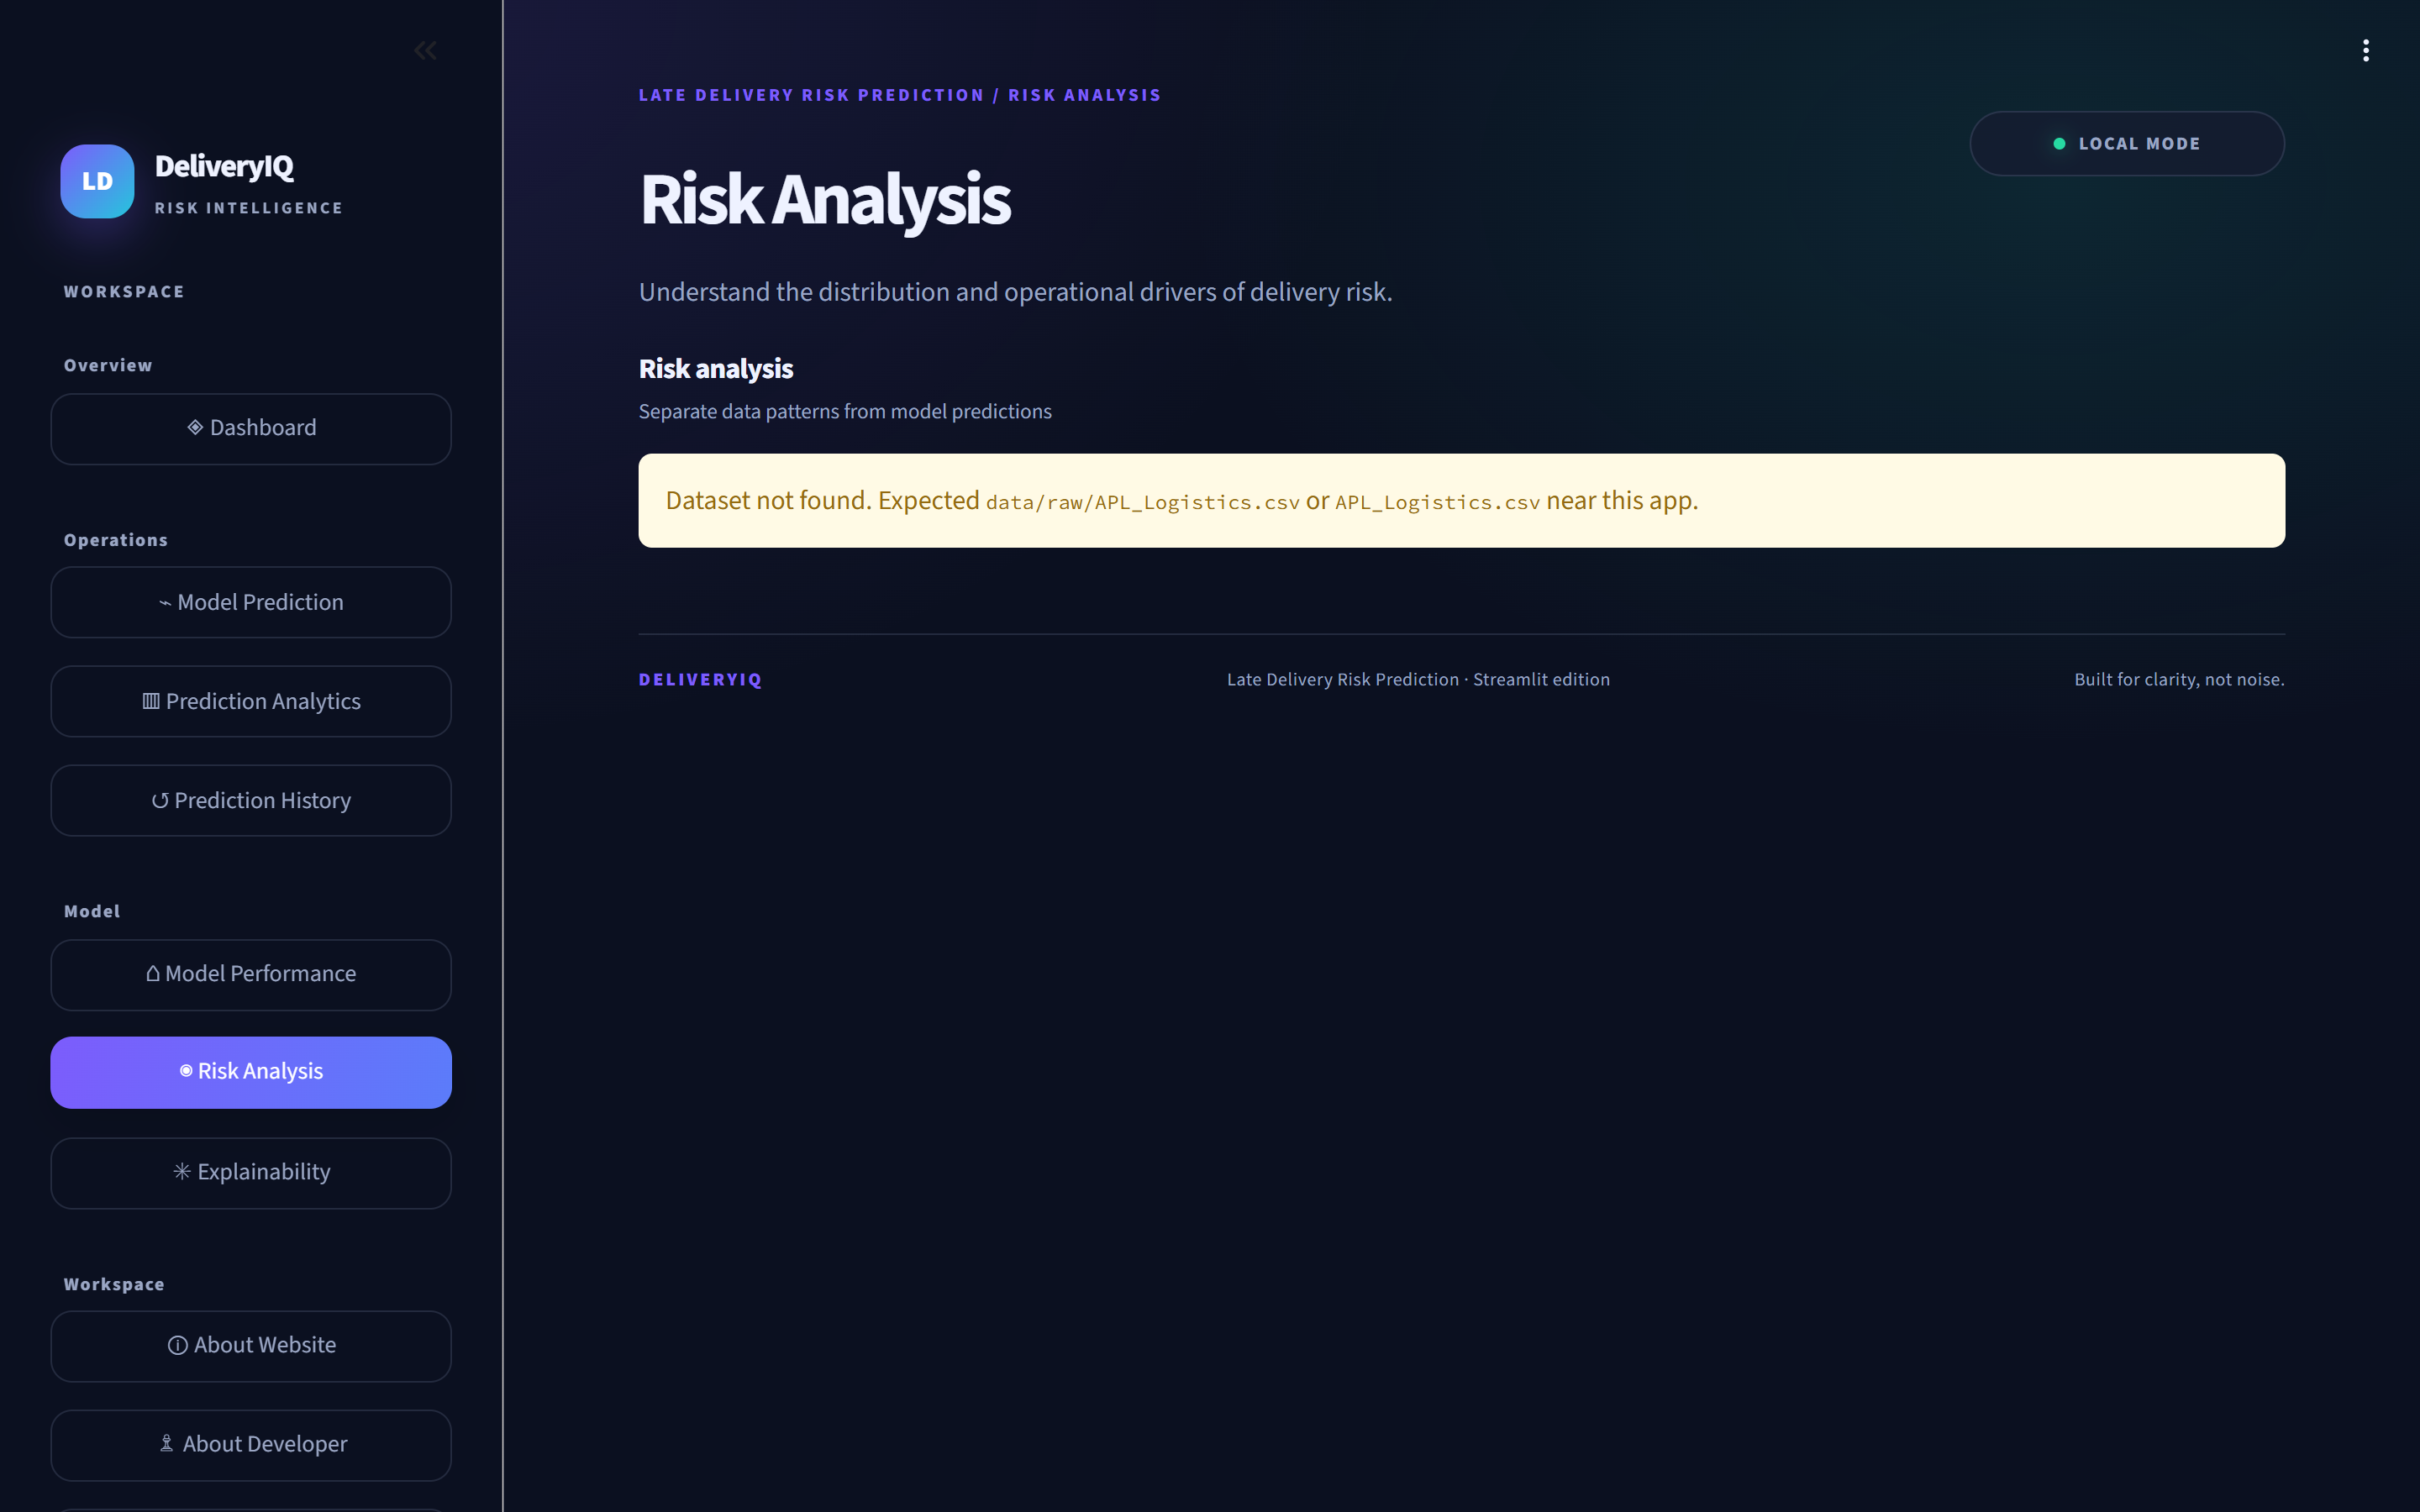
\includegraphics[width=\columnwidth]{figures/risk_analysis.png}
\caption{Risk Analysis view illustrating empirical delivery failure rates across logistics transportation modes.}
\label{fig:web_risk}
\end{figure}

\begin{figure}[htbp]
\centering
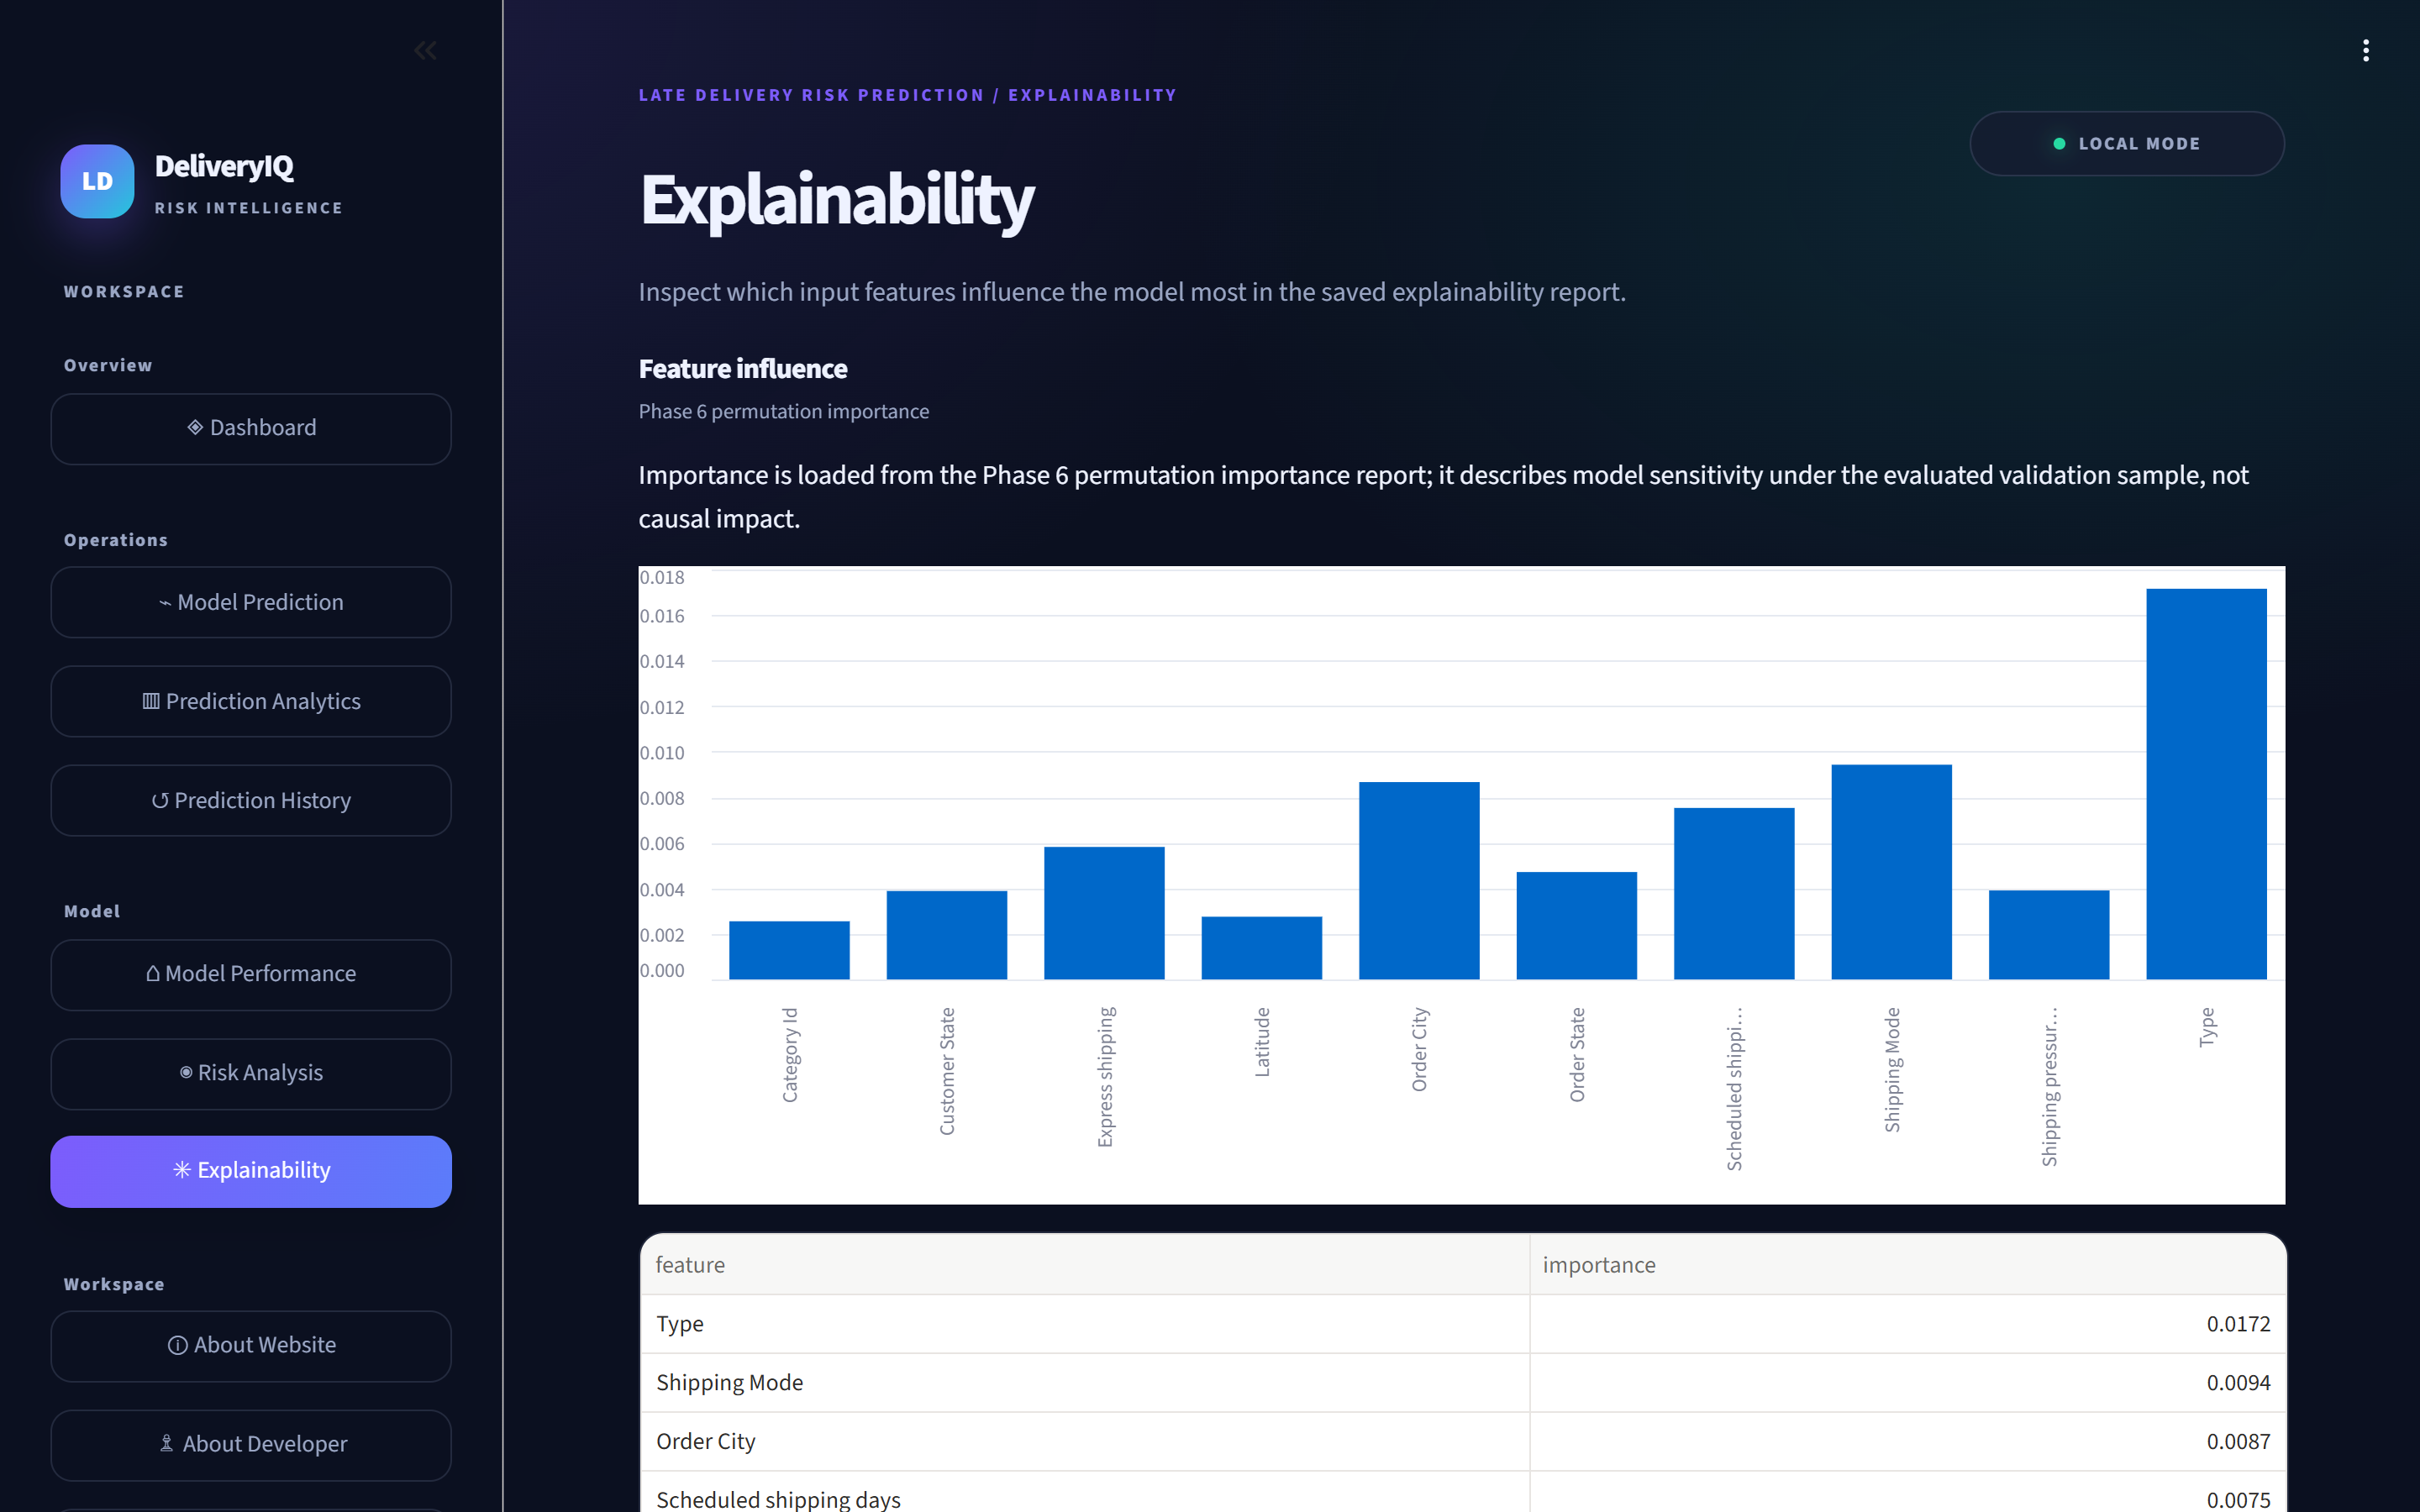
\includegraphics[width=\columnwidth]{figures/explainability.png}
\caption{Explainability view presenting global permutation feature importances for operational transparency.}
\label{fig:web_exp}
\end{figure}

\begin{figure}[htbp]
\centering
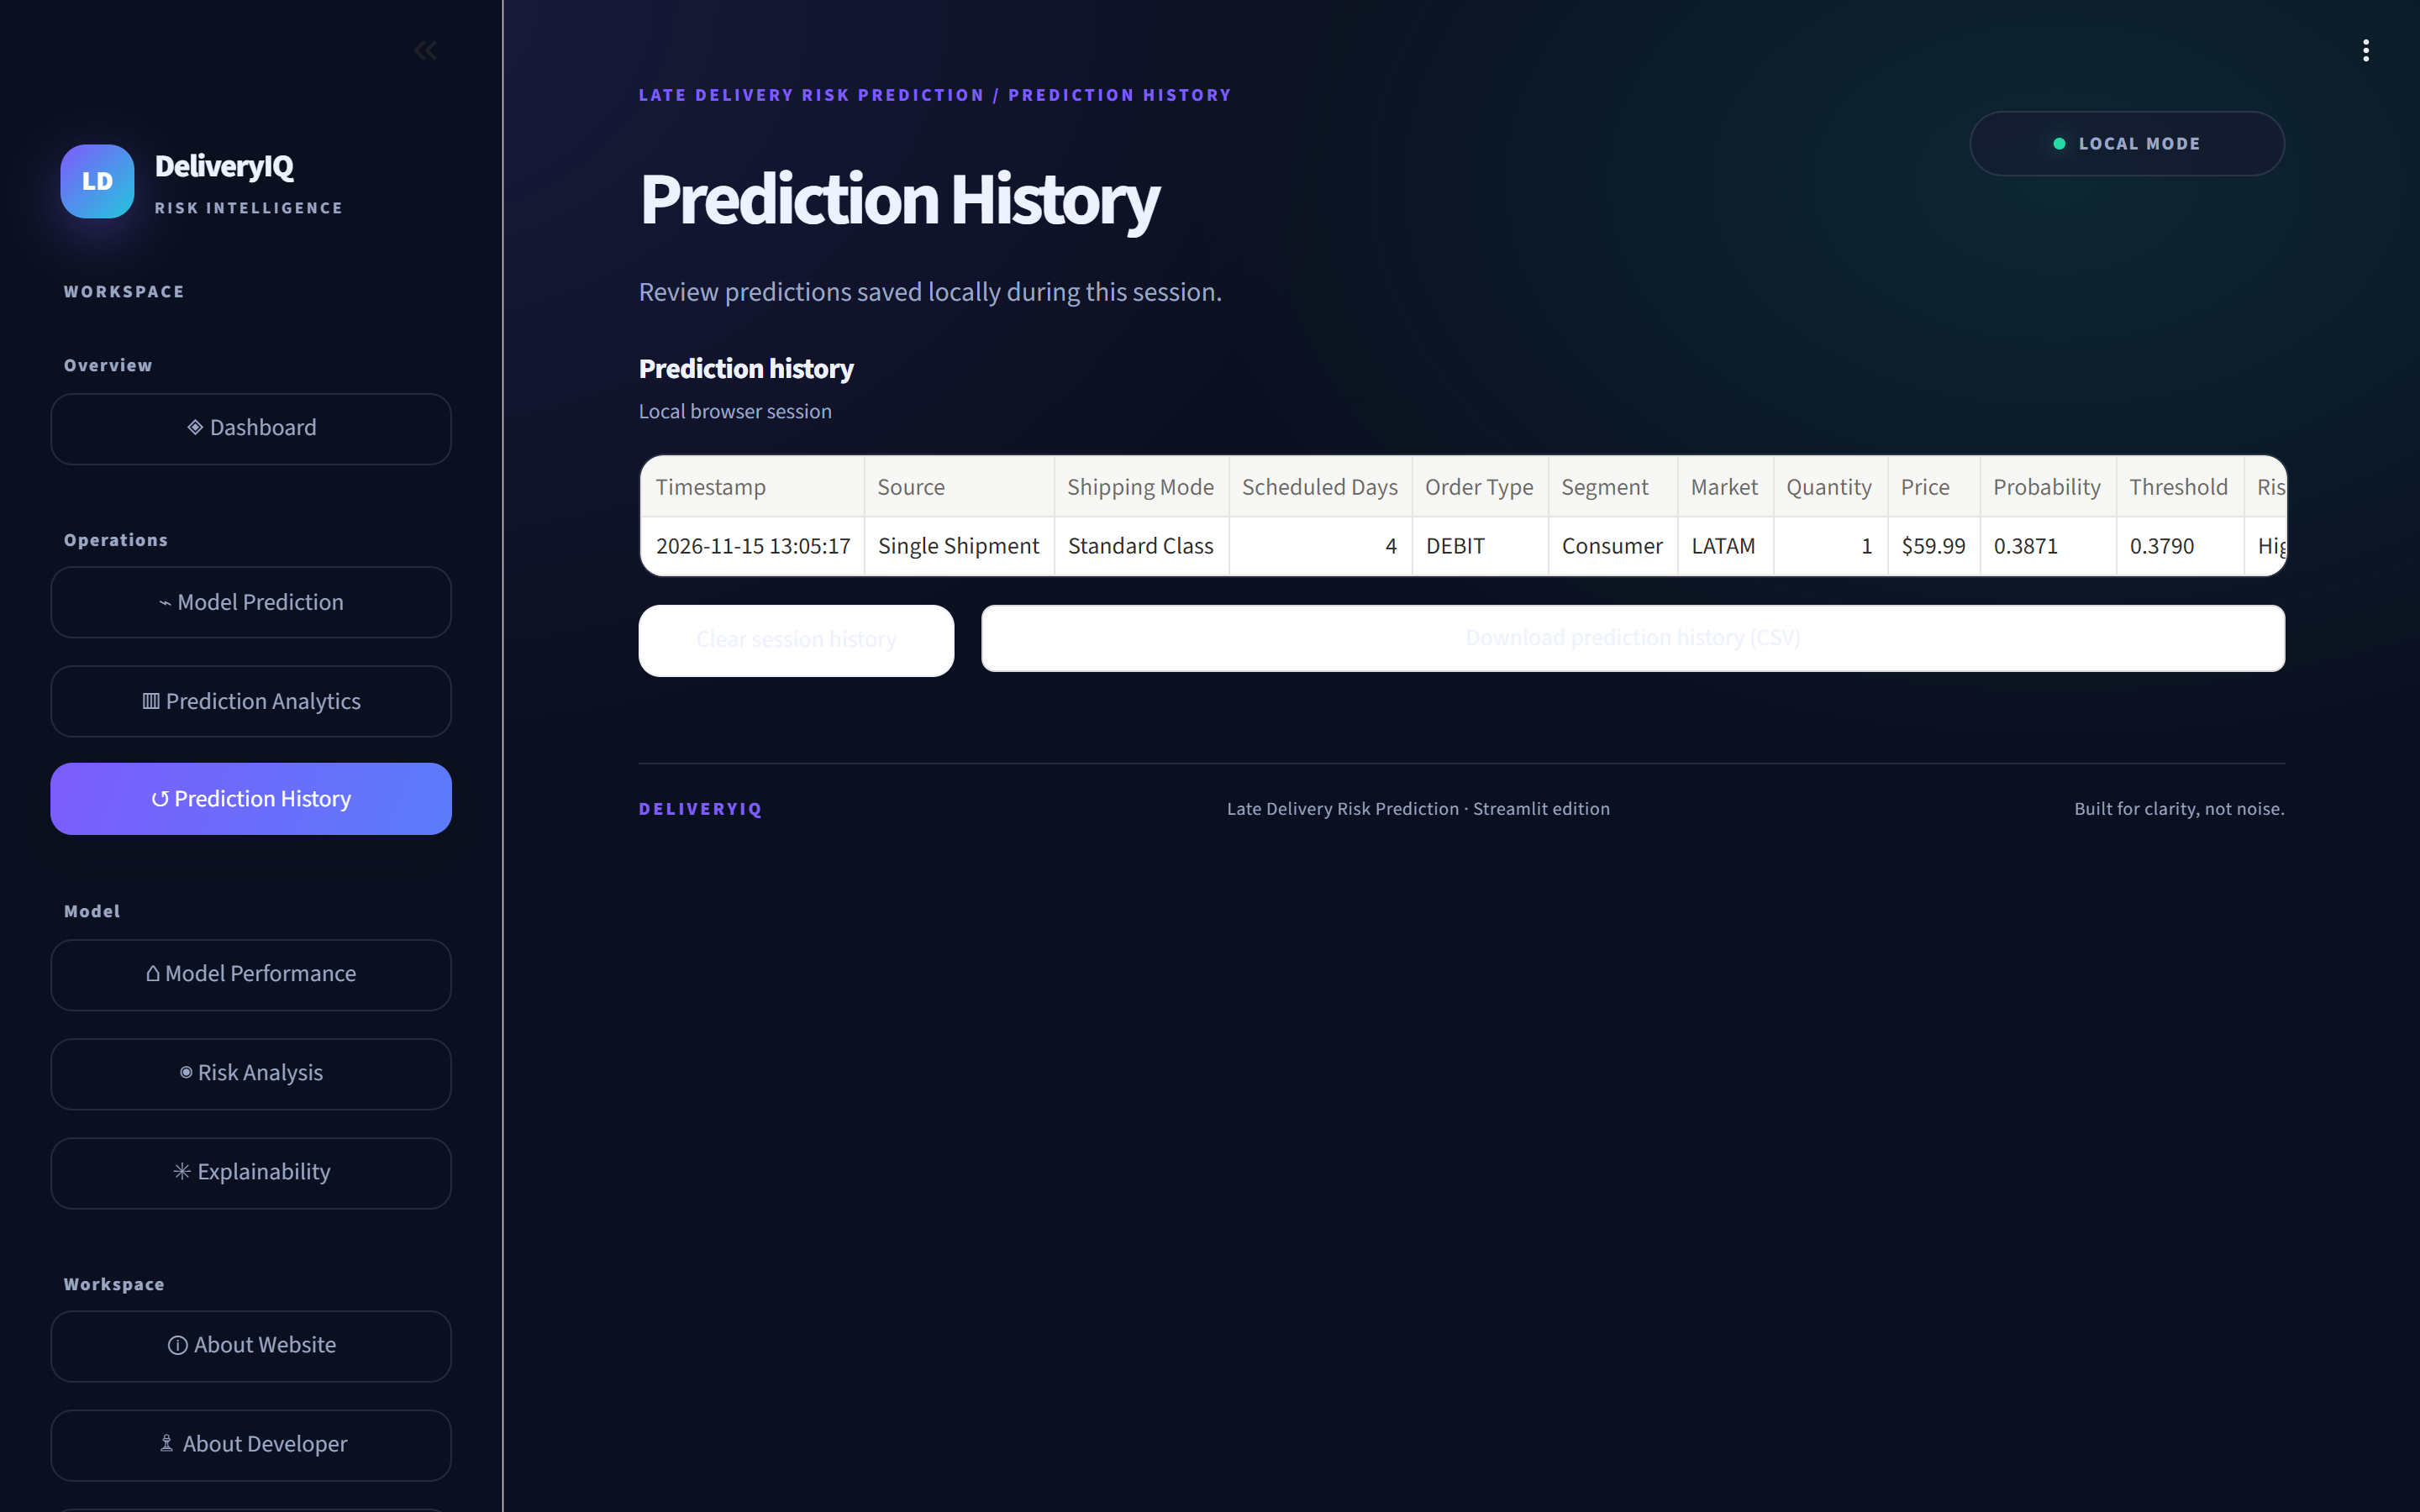
\includegraphics[width=\columnwidth]{figures/prediction_history.png}
\caption{Prediction History audit log recording timestamps, inputs, probability estimates, and decisions across assessments.}
\label{fig:web_hist}
\end{figure}

\begin{figure}[htbp]
\centering
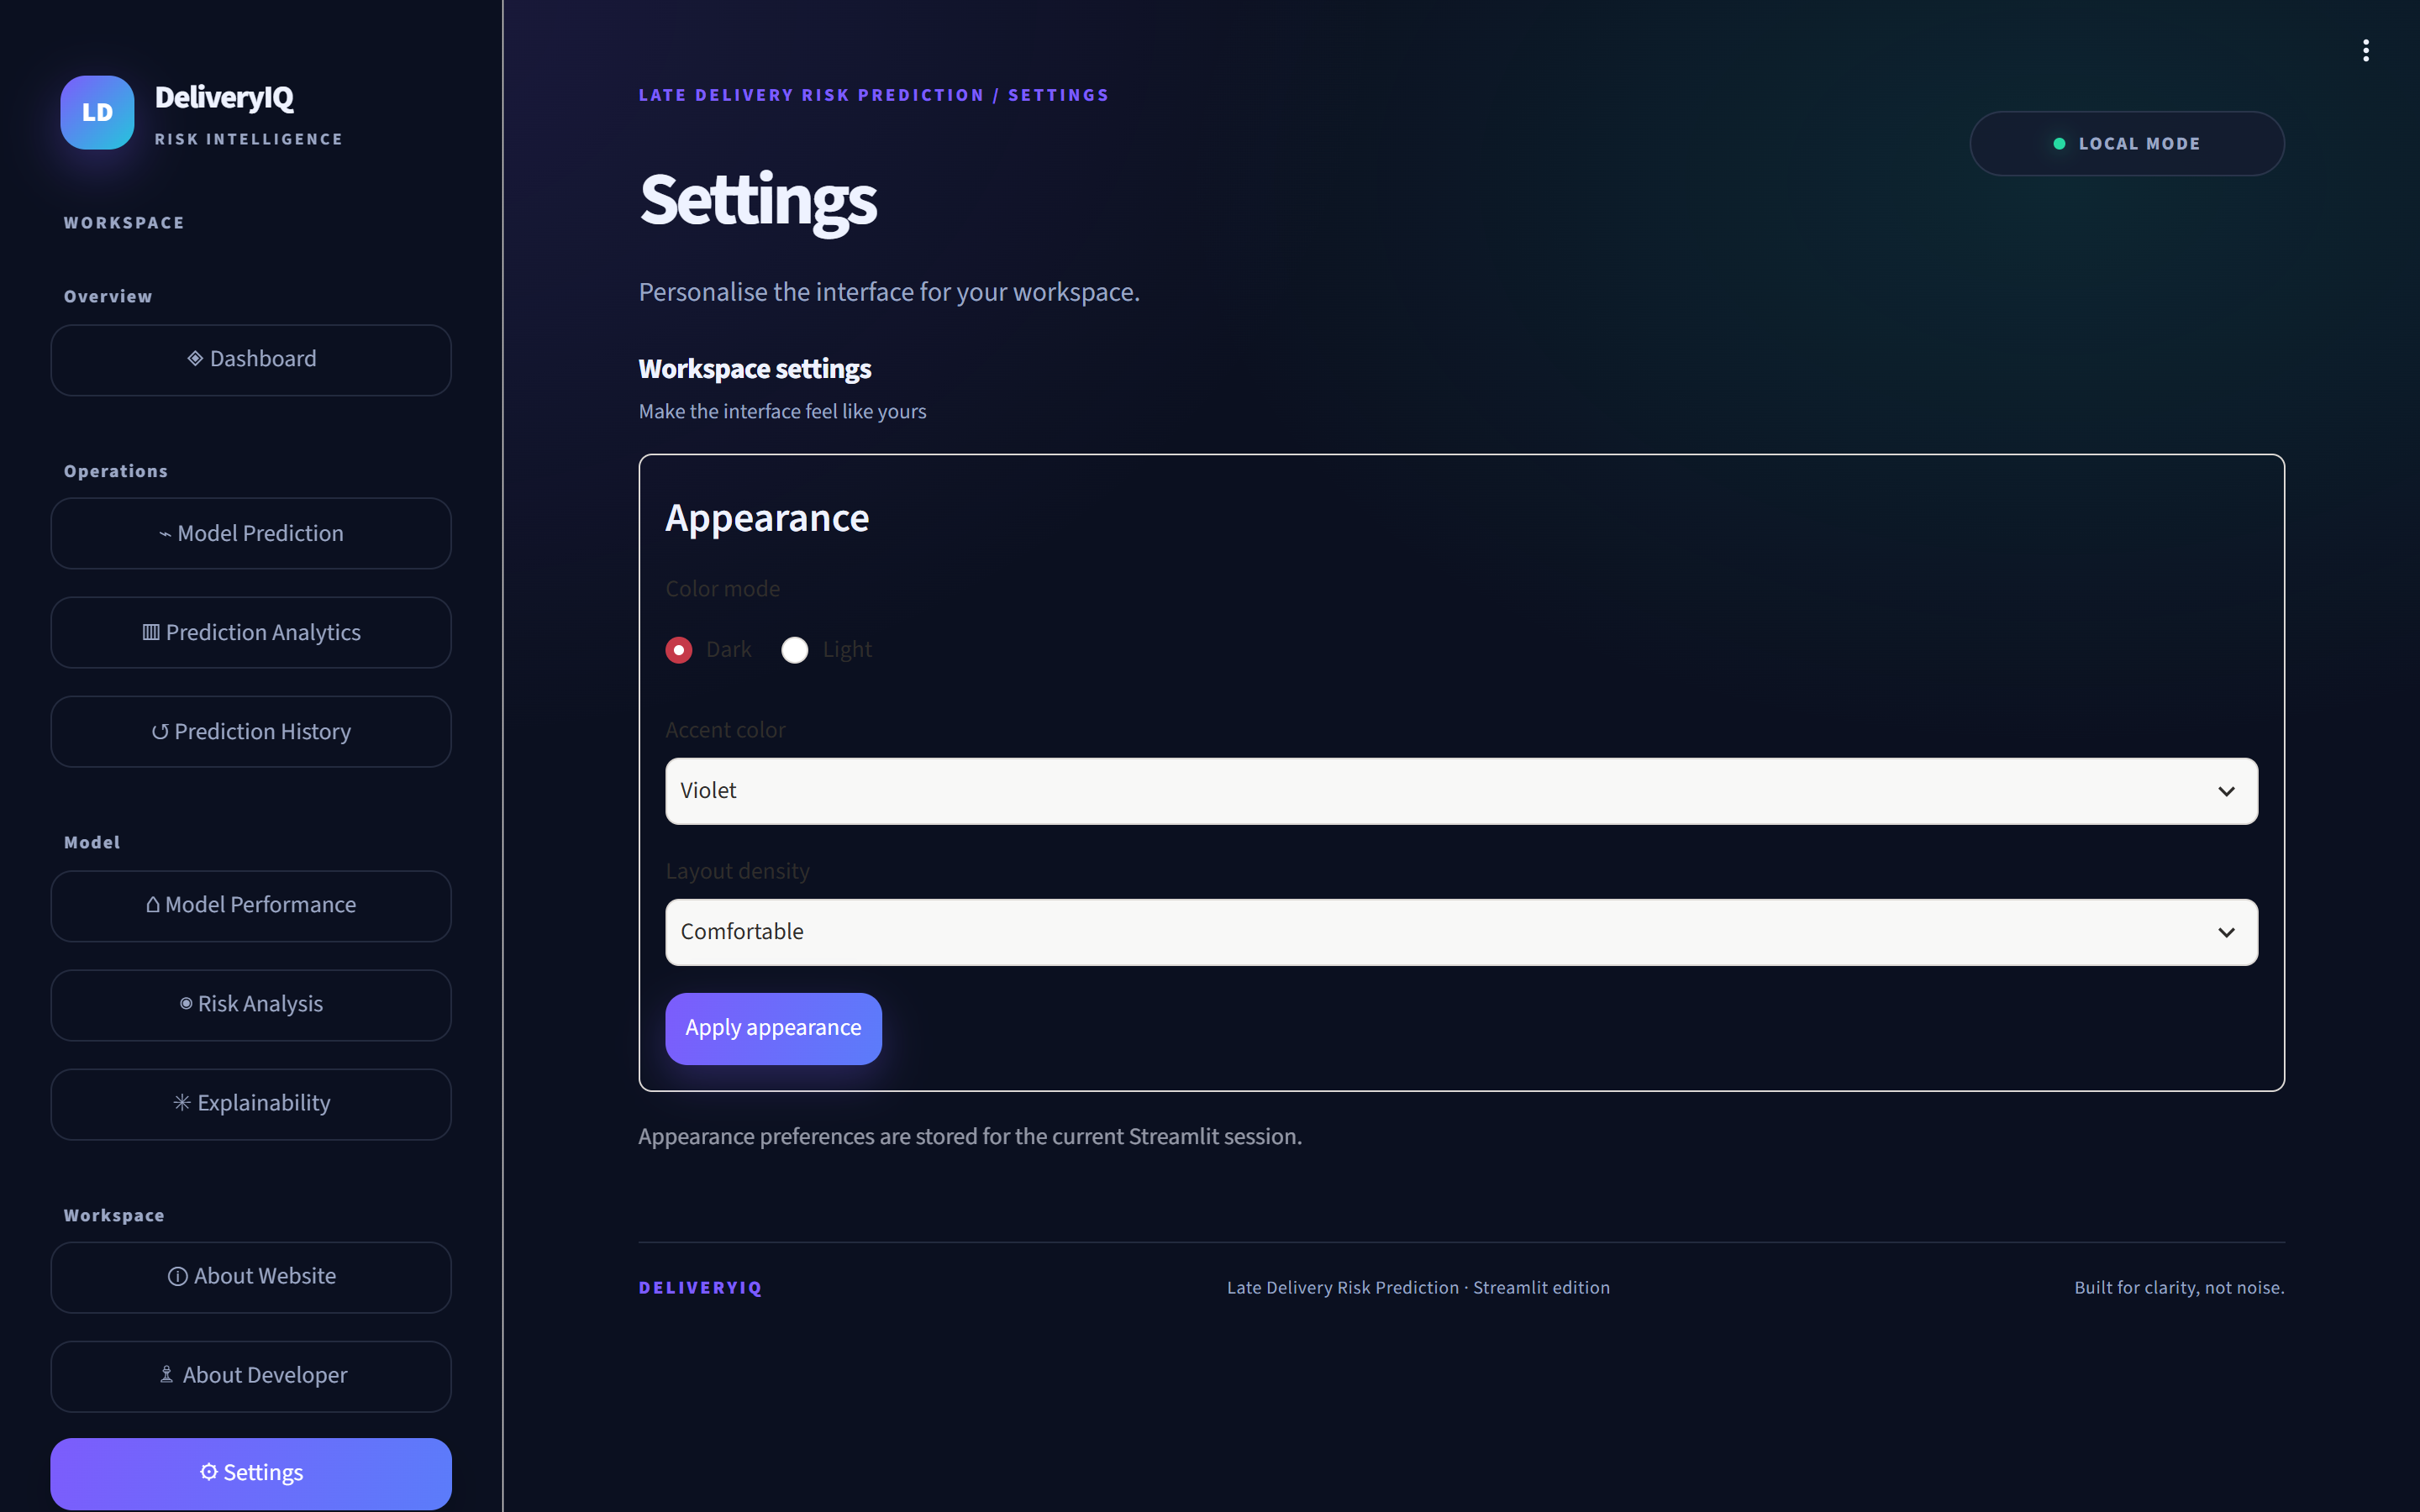
\includegraphics[width=\columnwidth]{figures/settings_page.png}
\caption{Workspace Settings interface for visual customization and appearance configuration.}
\label{fig:web_settings}
\end{figure}

\section{System Architecture and Deployment}
\label{sec:architecture}

\subsection{End-to-End Pipeline Implementation}
Fig.~\ref{fig:system_arch} illustrates the comprehensive architectural topology. The production inference pipeline is encapsulated within the \texttt{Phase5ModelAdapter} class, which couples the fitted \texttt{ColumnTransformer} and \texttt{RandomForestClassifier} into a single serialized bundle (\texttt{selected\_model\_bundle.joblib}).

\subsection{Cross-Version Imputer Compatibility Auto-Healing}
A critical production engineering challenge solved during deployment involved cross-version deserialization anomalies within Scikit-learn's \texttt{SimpleImputer}. While Scikit-learn versions $1.4.0$ through $1.6.x$ rely on the private attribute \texttt{\_fill\_dtype} during \texttt{transform()}, Scikit-learn $1.7.0+$ transitioned to \texttt{\_fit\_dtype}. When unpickling older bundles across heterogeneous cloud container environments, missing attributes trigger fatal \texttt{AttributeError} crashes.

DeliveryIQ implements an automated recursive healer within \texttt{model\_adapter.py} that inspects all nested pipeline transformers upon initialization:
\begin{equation}
\texttt{attr}_{\text{dtype}} = \operatorname{resolve}(\texttt{\_fill\_dtype}, \texttt{\_fit\_dtype}, \texttt{statistics\_})
\end{equation}
The adapter guarantees that both attributes are populated dynamically before \texttt{transform()} is invoked, ensuring permanent cross-version stability across Python and Scikit-learn cloud runtimes.

\section{Practical Decision-Support Framework}
\label{sec:decision_framework}

\subsection{Operational Dispatch Playbook}
To translate risk probabilities into tangible business value, DeliveryIQ establishes a multi-tiered operational dispatch playbook:
\begin{itemize}
    \item \textbf{Tier 1: Critical Risk ($\hat{p} \ge 0.65$):} Mandatory dispatch hold. Warehouse coordinator switches carrier tier from ground to air freight or splits multi-item pallets into regional fulfillment hubs.
    \item \textbf{Tier 2: High Risk ($\tau^* \le \hat{p} < 0.65$):} Accelerated dock priority. The shipment is prioritized for immediate same-day packing, staging, and early carrier pickup.
    \item \textbf{Tier 3: Moderate Risk ($0.30 \le \hat{p} < \tau^*$):} Monitored transit. Standard fulfillment proceeds, with automated webhook tracking alerts enabled.
    \item \textbf{Tier 4: Low Risk ($\hat{p} < 0.30$):} Standard fulfillment with normal shipping timelines.
\end{itemize}

\subsection{Summary of Research Question Findings}
Table~\ref{tab:rq_mapping} maps each defined research question to its empirical finding.

\begin{table}[htbp]
\caption{Mapping of Research Questions to Empirical Findings}
\label{tab:rq_mapping}
\centering
\begin{tabularx}{\columnwidth}{lX}
\toprule
\textbf{Research Question} & \textbf{Core Empirical Finding} \\
\midrule
\textbf{RQ1:} Leakage-Free Preprocessing & Purging post-shipment columns eliminates artificial 99\% inflation, yielding a valid pre-shipment baseline (63.65\% accuracy, 76.22\% ROC-AUC). \\
\addlinespace
\textbf{RQ2:} Engineered Features & Shipping pressure and express indicators rank among top predictive drivers, capturing physical dock constraints. \\
\addlinespace
\textbf{RQ3:} Model Comparison & Random Forest decisively outperforms linear Logistic Regression (+10.8\% ROC-AUC), handling non-linear categorical interactions. \\
\addlinespace
\textbf{RQ4:} Threshold Optimization & Shifting threshold to $\tau^* = 0.3790$ boosts delay recall from 57.22\% to 85.20\%, aligning with supply chain risk asymmetry. \\
\addlinespace
\textbf{RQ5:} Interactive Platform & DeliveryIQ provides real-time single-order scoring, batch CSV processing, and explainability via Streamlit Cloud. \\
\bottomrule
\end{tabularx}
\end{table}

\section{Limitations and Threats to Validity}
\label{sec:limitations}

While DeliveryIQ demonstrates strong predictive performance, several limitations must be acknowledged:
\begin{enumerate}
    \item \textbf{Absence of Real-Time Weather/Traffic Signals:} The dataset lacks dynamic, real-time external covariates, such as adverse meteorological storm tracks, port terminal labor strikes, or highway congestion telemetry.
    \item \textbf{Historical Snapshot Constraint:} Stratified splitting was utilized because the public DataCo dataset lacks continuous, monotonic multi-year timestamps required for strict walk-forward temporal cross-validation.
    \item \textbf{Non-Causal Feature Reliance:} Permutation feature importances establish statistical association rather than strict causal mechanisms.
\end{enumerate}

\section{Future Work}
\label{sec:future_work}

Future extensions of the DeliveryIQ framework will focus on:
\begin{itemize}
    \item Incorporating real-time GPS telematics and live weather API webhooks into the inference adapter.
    \item Deploying continuous model monitoring for covariate shift and concept drift detection using Evidently AI or MLflow.
    \item Implementing conformal prediction intervals to attach rigorous mathematical confidence bounds to predicted probabilities.
\end{itemize}

\section{Conclusion}
\label{sec:conclusion}

This paper presented \textbf{DeliveryIQ}, an end-to-end Machine Learning decision-support framework for pre-shipment late delivery risk prediction in global supply chain operations. By enforcing strict data leakage prevention across 180,519 multimodal logistics transactions, synthesizing domain-informed transit pressure features, and optimizing decision thresholds for cost-asymmetric logistics environments ($\tau^* = 0.3790$), our ensemble Random Forest achieves $85.20\%$ recall and $76.22\%$ ROC-AUC on held-out test data. The operationalization of this pipeline into an accessible Streamlit web application with transparent global and local explainability provides logistics teams with an actionable, forward-looking decision-support platform that transforms passive historical reporting into proactive dispatch intervention.

\section*{Acknowledgment}
The author gratefully acknowledges Lovely Professional University for providing the academic and technological resources supporting this research.

\bibliographystyle{IEEEtran}
\bibliography{references}

\end{document}
